% Kandidate prosimo, da nam posredujejo predloge za izbolj''save tega vzorca 
% na elektronski naslov Fizikalne knji''znice: fiz.knjiz@fmf.uni-lj.si.
%-----------------------------------------------------------------------------------------
%        METAPODATKI
%-----------------------------------------------------------------------------------------

\begin{filecontents*}{\jobname.xmpdata}
\Title{PREKLOPI MED TOPOLOŠKIMA FAZAMA V NEUREJENEM SU-SCHRIEFFER-HEEGERJEVEM MODELU}			                %%% vnesite svoj naslov magistrskega dela
\Author{Andrej Kolar - Požun}					                %%% vnesite svoje ime in priimek
\Keywords{topološki izolator\sep model SSH\sep nered\sep Andersonova lokalizacija\sep preklop} %%% vnesite svoje ključne besede
\Subject{Fizika}	
\end{filecontents*}

%-----------------------------------------------------------------------------------------

\documentclass[longbibliography,slovene,a4paper,12pt]{book}

\usepackage[slovene]{babel}    
\usepackage[utf8]{inputenc}
\usepackage{amsfonts}
\usepackage[T1]{fontenc}
\usepackage[pdftex]{graphicx}
\usepackage{fancyhdr}
\usepackage[sort, numbers]{natbib}
\usepackage{acro}
\usepackage[nottoc,numbib]{tocbibind}
\usepackage{amsmath}
\usepackage{graphicx}
\usepackage{amsthm}
\usepackage{subcaption}
\usepackage{amssymb}
\usepackage{caption}
\usepackage{float}
\usepackage{physics}
\usepackage{multicol}
\newtheorem*{theorem*}{Birkhoffov izrek}
\newdimen\visina
\newdimen\sirina 

%---------------------------------------------------------------------------------------------
%        PDF/A
%---------------------------------------------------------------------------------------------

\usepackage{xmpincl}
\usepackage[a-1b]{pdfx}       

%----------------------------------------------------------------------------------------------

\usepackage{filecontents}
\usepackage{hyperref}
\usepackage{url}
\usepackage[a4paper,inner=3.5cm,outer=2.5cm,top=2.5cm,bottom=2.5cm,pdftex]{geometry}
\usepackage[titletoc,title]{appendix}
\usepackage{epstopdf}
\usepackage{makeidx}
\pagestyle{fancy}
\setlength{\headheight}{15pt}
\usepackage{enumitem}
\usepackage{underscore}
\usepackage{tocloft}
\renewcommand{\cftpartleader}{\cftdotfill{\cftdotsep}} 
\renewcommand{\cftchapleader}{\cftdotfill{\cftdotsep}} 

\makeindex

\def\epsfg#1#2{\epsfig{file=#1.eps,width=#2}}
\def\legendamp#1#2{\vbox{\hsize=#1\caption{\small #2}}}

\setcounter{topnumber}{4}
\setcounter{bottomnumber}{4}
\setcounter{totalnumber}{5}
\renewcommand{\topfraction}{0.99}
\renewcommand{\bottomfraction}{0.99}
\renewcommand{\textfraction}{0.0}
\setlength{\tabcolsep}{10pt}
\renewcommand{\arraystretch}{1.5}

\def\bi#1{\hbox{\boldmath{$#1$}}}
\let\oldvec\vec
\def\vec#1{\mbox{\boldmath$#1$}}
\def\pol{{\textstyle{1\over2}}}
\def\svec#1{\mbox{{\scriptsize \boldmath$#1$}}}


%----------------------------------------------------------------------------------------
%    SUMNIKI
%----------------------------------------------------------------------------------------
%% Za pisanje sumnikov imamo tri moznosti:
%%   --- vnasamo jih neposredno v kodnem sistemu UTF-8 
%%   --- pisemo jih z latexovim ukazom, ki je namenjen natanko temu,
%%       in sicer kot \v{c}, \v{s}, \v{z}, \v{C}, \v{S}, v{\Z} ali
%%       malo manj pregledno kot \v c, \v s, \v z, \v C, \v S, \v Z,
%%   --- pisemo jih kot "c, "s, "z, "C, "S, "Z), vendar tedaj potrebujemo
%%       spodaj zapisani macro, ki znaku " pripise vlogo `izdelave' sumnika:
\catcode`\"=\active\def"#1{\v{#1}}
%%       torej \v{S}krjan\v{c}ek == \v Skrjan\v cek == "Skrjan"cek
%% Pozor: narekovaj potem ne smemo vec pisati kot " ampak kot `` in '',
%%       torej: "Skrjan"cek je "civkal ``"ci-"ci-"ci''.
%
%------------------------------------------------------------------------------------------

\begin{document}

%--------------------------------------------------------------------------------------
%       NASLOVNA STRAN
%-----------------------------------------------------------------------------------

\pagestyle{empty}
\begin{center}

{\large UNIVERZA V LJUBLJANI\\
FAKULTETA ZA MATEMATIKO IN FIZIKO\\
ODDELEK ZA FIZIKO\\
MATEMATIČNA FIZIKA\\}


\vspace{4cm}


{\Large Andrej Kolar - Požun\\}

\vspace{10mm}

{\bf \Large PREKLOPI MED TOPOLOŠKIMA FAZAMA V NEUREJENEM SU-SCHRIEFFER-HEEGERJEVEM MODELU}\\
\vspace{5mm}
{\large Magistrsko delo}\\




\vfill



{\large MENTOR: doc. Tomaž Rejec\\
SOMENTORICA: asist. Lara Ulčakar\\


\vspace{2cm}
Ljubljana, 2020}

\end{center}

%--------------------------------------------------------------------------
%        ZAHVALA (NEOBVEZNO)
%--------------------------------------------------------------------------

\cleardoublepage
\mbox{}
\vfill
{\Large \bf Zahvala}
\vspace{1cm}\\
Za pomoč in nasvete pri magistrskem delu bi se rad zahvalil mentorju Tomažu Rejcu in somentorici Lari Ulčakar.
Za neprestano podporo pri študiju pa se zahvaljujem družini in prijateljem. Hvala!
%------------------------------------------------------------------------
%         IZVLECEK
%-----------------------------------------------------------------------

\cleardoublepage
\begin{center}
{\bf Preklopi med topološkima fazama v neurejenem Su-Schrieffer-Heegerjevem modelu}\\[3mm]
{\sc  Izvle"cek}
\end{center}
\vspace{10mm}
V delu obravnavamo neurejen Su-Schrieffer-Heegerjev model. V takem sistemu lahko med topološkima fazama prehajamo tudi s spreminjanjem jakosti nereda. Kritična točka tega prehoda je zaznamovana z delokalizacijo stanja z energijo nič, v njeni okolici pa se nahaja široko območje brez energijske reže. Glavnina dela je posvečena proučevanju počasnih preklopov Hamiltonjana preko omenjene kritične točke. Med preklopom se pojavijo ekscitacije v prevodnem pasu, katerih število skalira kot potenčna funkcija hitrosti preklopa z logaritemskim popravkom. Potenčno odvisnost opazimo tudi pri skaliranju energij najvišje vzbujenih elektronov s hitrostjo preklopa. Pri dovolj počasnih preklopih se pojavi univerzalna časovna odvisnost števila ekscitacij od časa. Delo zaključimo s podrobnejšo analizo posameznih ekscitacij in ugotovimo, da preklopljeno stanje praviloma preide v le dve stanji v prevodnem pasu. \\[10mm]
{\bf Klju"cne besede: topološki izolator, model SSH, nered, Andersonova lokalizacija, preklop.}\\[3mm]

\cleardoublepage

 \foreignlanguage{english}{  %  angleski delilni vzorci
\begin{center}
{\bf Quenches Between Topological Phases in a Disordered Su-Schrieffer-Heeger Model}\\[3mm]
{\sc  Abstract}
\end{center}
\vspace{10mm}
We consider a disordered Su-Schrieffer-Heeger model. In such a system a transition between topological phases is also possible by changing the strength of the disorder. The critical point of this phase transition coincides with the delocalization of the zero energy state, while in its neighbourhood we observe a wide area without the energy gap. The main part of our work is devoted to the study of slow Hamiltonian quenches over the previously mentioned critical point. During the quench, excitations in the conduction band appear with their number scaling as a power law of the quench speed with a logarithmic correction. A power law scaling is also observed in the dependence of the highest excited electrons' energies on the quench speed. For slow enough quenches we find universal dependence of the number of excitations on time. We conclude with a detailed analysis of individual excitations and notice that the quenched state generally transitions to only two states in the conduction band.\\[10mm]
{\bf Keywords: topological insulator, the SSH model, disorder, Anderson localization, quench.}\\[3mm]
}

%------------------------------------------------------------------------
%        KAZALO
%----------------------------------------------------------------------

\cleardoublepage
\tableofcontents

%------------------------------------------------------------------------
%       OSREDNJI DEL
%-------------------------------------------------------------------------

\pagestyle{fancy}
\fancyhead[CE,RE]{}
\fancyhead[LO,CO]{}
\fancyhead[LE]{\textbf{\nouppercase{\leftmark}}}
\fancyhead[RO]{\textbf{\nouppercase{\rightmark}}}

%\input{Uvod}

\chapter{Uvod}
\label{chUv}
Že dalj časa je znano, da lahko fizikalne sisteme v fiziki trdne snovi klasificiramo na prevodnike in izolatorje, odvisno od obstoja energijske reže med zasedenimi in nezasedenemi nivoji v spektru Hamiltonjana. V zadnjih desetletjih pa so raziskovalno popularni posebni tipi izolatorjev - topološki izolatorji \cite{madzar, yoichi}. Te lahko nadalje klasificiramo v različne topološke faze, katerih ureditveni parameter je celoštevilska topološka invarianta. Ti materiali so zanimivi, ker se topološke invariante ne spreminjajo med adiabatnimi transformacijami, kar pomeni, da so topološke faze robustne: zvezne transformacije, ki ne zaprejo energijske reže in ohranjajo pomembne simetrije modela, ne morejo povzročiti prehoda med topološkimi fazami. V topoloških izolatorjih ima pomembno vlogo rob materiala, kjer se za razliko od običajnih materialov pojavijo netrivialna robna stanja. Kljub temu, da se v notranjosti material obnaša kot izolator, so namreč lahko na robu prisotna prevodna stanja, katerih število je preko tako imenovane korespondence notranjost-rob povezano s topološko invarianto topološkega izolatorja. Iz robustnosti topološke invariante sledi tudi robustnost prevodnih robnih stanj, kar pomeni, da lahko rob topološkega izolatorja predstavlja dober prevodnik, čeprav so v materialu prisotne nečistoče. Topološki fizikalni sistemi so nasploh popularna raziskovalna tema, saj temelji ena izmed najbolj razširjenih idej za izgradnjo kvantnega računalnika na topoloških kubitih, ki jih topološka narava ščiti pred dekoherenco \cite{computer}.

V tem delu se bomo posvetili enodimenzionalnemu topološkem izolatorju z nečistočami (neredom). Prisotnost nereda lahko lastnosti obravnavanega sistema bistveno spremeni: znano je na primer, da se lahko že pri zelo majhnem neredu vsa lastna stanja lokalizirajo \cite{anders}. Povedali smo že, da so sicer topološke faze robustne na nečistoče v materialu, vendar to velja le, ko te niso premočne. Ko so premočne, preide sistem v trivialno fazo.
Osredotočili se bomo na preklop Hamiltonjana preko take kritične točke. S tem imamo v mislih časovni razvoj stanja s časovno odvisnim Hamiltonjanom, saj bomo jakost nereda s časom povečevali. Začeli bomo s stanjem v topološki fazi in s povečevanjem jakosti nereda končali v trivialni fazi. Zaradi končne hitrosti preklopa in zapiranja energijske reže v okolici kritične točke se pri tem v prevodnem pasu pojavijo ekscitacije. Glavni cilj dela je raziskati skaliranje števila ekscitacij v odvisnosti od hitrosti preklopa. Motivacija za to je Kibble-Zurekov mehanizem \cite{kibble}, ki predvideva potenčno skaliranje in potenco poveže s kritičnimi eksponenti faznega prehoda. Kibble-Zurekov mehanizem sicer primarno opisuje preklope med navadnimi (torej ne topološkimi) fazami, kjer pride pri faznem prehodu do zloma simetrije, vendar so raziskave  \cite{uvod1, uvod2, lara1} pokazale, da se podobno obnašanje pojavi tudi v topoloških sistemih.

V naslednjih dveh poglavjih bomo predstavili potrebno teoretično predznanje za razumevanje obravnavanega modela.
Začeli bomo z najenostavnejšim modelom topološkega izolatorja - Su-Schrieffer-Heegerjevim (SSH) modelom \cite{SSH}. Ta nam bo kljub svoji preprostosti dal vpogled v nekaj znanih lastnosti topoloških izolatorjev. Na primeru modela SSH se bomo, na primer, seznanili s konceptom topoloških faz in adiabatskih deformacij. V nadaljevanju bomo pogledali še teorijo fizikalnih sistemov z neredom, kjer bomo spoznali pojav Andersonove lokalizacije.

V četrtem poglavju bomo predstavili model neurejenega enodimenzionalnega topološkega izolatorja, ki bo osrednji predmet raziskave v tem magistrskem delu. Najprej si bomo ogledali fazni diagram takega modela, potem pa preučili še njegov spekter. Zatem bomo predstavili še numerično metodo za izračun časovnega razvoja elektronskih stanj, ki jo bomo uporabljali pri preklapljanju.

Končno bomo v petem poglavju predstavili rezultate preklapljanja. Najprej se bomo osredotočili na funkcijsko odvisnost celotnega števila ekscitacij med preklapljanjem, nato pa raziskali še njihovo energijsko porazdelitev, proti koncu pa si bomo ogledali še podrobnejše obnašanje posameznih ekscitacij.

\chapter{Topološki izolatorji}
\label{chMa}

\section{Model SSH}
Najpreprostejši model topološkega izolatorja je Su-Schrieffer-Heegerjev (SSH) model, ki obravnava enodimenzionalno Bravaisovo rešetko (verigo), kjer je osnovna celica sestavljena iz dveh mest, ki ju označimo s črkama A in B. V tem modelu obravnavamo - kot v modelu tesne vezi - elektron, ki skače med najbližjimi sosedi na verigi. Kot je razvidno iz slike \ref{fig:chain}, je skakanje med mestoma v isti osnovni celici določeno s sklopitvenim parameterom $v \in \mathbb{R}$, medtem ko je skakanje med sosednjimi mesti iz različnih osnovnih celic določeno s (v splošnem različnim) parameterom $w \in \mathbb{R}$.
\begin{figure}[!h]
\centering
\begin{subfigure}{.9\textwidth}
\includegraphics[width=\linewidth]{Figures/MySSHChain.pdf}
\end{subfigure}
\caption{atomska veriga, ki ustreza modelu SSH. Svetlo in temno sivi krogi ustrezajo mestom tipa A in B. Osnovna celica je označena z modro, črtkano črto. Vez med mestoma v isti osnovni celici je označena s črto s pikicami, medtem ko je vez med različnimi osnovnimi celicami označena s črto s prečnimi črtkami. Veriga na sliki je sestavljena iz petih osnovnih celic. }
\label{fig:chain}
\end{figure}
Če prevedemo zgornje napisano v Hamiltonski opis, dobimo Hamiltonjan modela SSH \cite{SSH}:
\begin{equation}
\hat{H} = v \sum_{m=1}^{\frac{N}{2}} \left( |m, B \rangle \langle m, A |  + \textup{h.c.} \right) + w \sum_{m=1}^{\frac{N}{2}-1} \left( | m+1, A \rangle \langle m, B |  + \textup{h.c.} \right),
\end{equation}
kjer $|m , \alpha \rangle = |m \rangle \otimes | \alpha \rangle$, z $m=1,.., \frac{N}{2}$ in $\alpha \in \{A,B\}$, označuje stanje elektrona, ki je lokalizirano na podmreži $\alpha$ v $m$-ti osnovni celici. Število vseh mest v verigi je $N$, kar pomeni, da je osnovnih celic $\frac{N}{2}$.  Analogno razdelimo tudi naš Hamiltonjan na del, ki deluje na zunanjo prostorsko stopnjo $|m \rangle$ in na del, ki deluje na notranjo prostorsko stopnjo $| \alpha \rangle$: 
\begin{equation}
\hat{H} = v \sum_{m=1}^{\frac{N}{2}} \Big( |m \rangle \langle m| \otimes \hat{\sigma}_x +\textup{h.c.} \Big) + w \sum_{m=1}^{\frac{N}{2}-1} \left( | m+1\rangle \langle m | \otimes \frac{\hat{\sigma}_x + i \hat{\sigma}_y}{2} + \textup{h.c.} \right),
\end{equation}
kjer sta $\hat{\sigma}_x$ in $\hat{\sigma}_y$ Paulijeva operatorja.

\subsection{Fizika translacijsko invariantnega sistema} \label{spomnimoTIS}
Za trenutek pozabimo na rob verige in se osredotočimo na njeno notranjost. Zanima nas torej dolg, sredinski del verige, ki prostorsko prevlada v termodinamski limiti $N \to \infty$. Ker fizika v notranjosti materiala ni odvisna od dogajanja na robu \cite{ashcroft}, lahko za njeno obravnavo izberemo najpreprostejše robne pogoje - periodične robne pogoje. Takšni robni pogoji ustrezajo translacijsko invariantnemu sistemu, za kar uvedimo oznako TIS. Hamiltonjan $\hat{H}_{\textup{TIS}}$, ki opisuje to fiziko, lahko torej dobimo iz prejšnjega Hamiltonjana, če vanj preprosto dodamo člen $w\ | 1, A \rangle \langle N/2, B|$  (in seveda njegovo hermitsko konjugiranko), ki opiše interakcijo med prvo in zadnjo osnovno celico prvotne verige, s čimer jo transformira v periodično verigo.
Iščemo $N$ lastnih stanj $|\Psi_n (k) \rangle$ z energijami $E_n(k)$:
\begin{equation}
\hat{H}_{\textup{TIS}} | \Psi_n (k) \rangle = E_n(k) | \Psi_n(k) \rangle.
\end{equation} 
V zgornji enačbi smo že zapisali energije in stanja kot funkcije Blochovega vektorja $k$, saj vemo, da velja za translacijsko invariantne sisteme Blochov teorem \cite{ashcroft}, ki pravi, da lahko lastna stanja napišemo v naslednji obliki:
\begin{equation}
| \Psi_n (k) \rangle = | k \rangle \otimes | u_n (k) \rangle.
\end{equation}
Vpeljali smo ravni val $|k\rangle$:
\begin{equation}
|k \rangle = \frac{1}{\sqrt{N/2}} \sum_{m=1}^{\frac{N}{2}} e^{imk} |m \rangle,
\end{equation}
kjer $k$ zavzame $\frac{N}{2}$ različnih vrednosti v prvi Brillouinovi coni.
Zdaj lahko definiramo še Hamiltonjan v recipročnem prostoru $\hat{H}(k) = \langle k | \hat{H}_{\textup{TIS}} | k \rangle$, ki deluje na notranjo prostorsko stopnjo:
\begin{equation}
\hat{H}(k) | u_n(k) \rangle = E_n(k) | u_n(k) \rangle.
\end{equation}
Če razvijemo notranji del valovne funkcije po podmrežni bazi $|u_n(k) \rangle = a_n(k) |A \rangle + b_n(k) | B \rangle$,
postane $\hat{H}(k)$ (hermitska) matrika $2 \times 2$ in jo lahko zapišemo kot linearno kombinacijo Paulijevih matrik in identitete:
\begin{equation} \label{spomnimo1}
H(k) = d_0 (k) \mathbb{I}+ d_x(k) \sigma_x + d_y (k) \sigma_y + d_z(k) \sigma_z.
\end{equation}
Iz koeficientov razvoja tvorimo vektor $\mathbf{d}(k) = (d_x (k), d_y (k) ,d_z (k) )$, iz katerega bomo dobili topološke lastnosti modela. Izkaže se, da je za model SSH $d_z(k)$ enak nič. Ko $k$ prepotuje prvo Brillouinovo cono, oriše vektor $\mathbf{d}(k)$ krivuljo v dvodimenzionalni ravnini $(d_x,d_y)$. Zaradi periodičnosti funkcije $\mathbf{d}(k)$ mora biti ta krivulja zanka, ki jo lahko topološko klasificiramo s celoštevilskim parametrom - ovojnim številom okoli izhodišča $\nu$ \cite{hatcher}. Kot bo razjasnjeno s primeri, nam ovojno število pove, kolikokrat se orientirana zanka "ovije"\   okoli izhodišča.
Konkretno lahko z eksplicitno konstrukcijo Hamiltonjana v recipročnem prostoru dobimo vektor:
\begin{equation}
\mathbf{d}(k) = (v + w \cos k, w \sin k, 0).
\end{equation}
Zanke, ki ustrezajo različnim izbiram parametrov $v, w$, lahko vidimo v drugi vrstici na sliki \ref{fig:examples}. Za $w < v$ imamo $\nu = 0$, medtem ko $w > v$ da $\nu=1$. Primer, ko velja $w=v$, je poseben, saj gre v tem primeru zanka $\mathbf{d}(k)$ skozi izhodišče, kar pomeni, da je ovojno število okoli izhodišča nedefinirano.
V prvi vrstici je na sliki \ref{fig:examples} prikazana disperzijska relacija za vsak obravnavan primer. Dobimo jo z diagonalizacijo Hamiltonjana v recipročnem prostoru, kar da:
\begin{equation}
E(k) = \pm \sqrt{v^2 + w^2 + 2 w v \cos k}
\end{equation}
Vidimo lahko, da je za primere $v \neq w$ prisotna končna energijska reža med prevodnim in valenčnim pasom, kar po definiciji ustreza izolatorju. Pri posebni točki $v=w$, kjer je ovojno število nedefinirano, se energijska reža zapre in sistem preide v prevodno stanje. Imamo torej dve možni izolatorski fazi, ki se razlikujeta po ureditvenem parameteru $\nu$. Primeru $\nu=0$ bomo rekli trivialna faza, medtem ko primer $\nu=1$ ustreza topološki fazi. Ovojno število je topološka invarianta v naslednjem smislu: ohranjajo ga zvezne deformacije (homotopije) zank, ki se izognejo izhodišču. Zvezen prehod med različnima izolatorskima fazama je torej možen le s prehodom skozi prevodno stanje, kar grafično pomeni, da gre med homotopijo zanka skozi izhodišče. K tej lastnosti modela se bomo kasneje vrnili v splošnejšem smislu.
\begin{figure}[!h]
\centering
\begin{subfigure}{.9\textwidth}
\includegraphics[width=\linewidth]{Figures/GapAndTopology.png}
\end{subfigure}
\caption{v prvi vrstici je prikazana disprezijska relacija za različne kombinacije parametrov $v$ in $w$. V drugi vrstici so narisane zanke $\vec{d}(k)$ v ravnini $(d_x , d_y)$. Prva stolpca ustrezata $\nu = 0$, zadnja ustrezata $\nu = 1$, medtem ko gre v sredinskem zanka skozi izhodišče in $\nu$ ni definiran. Vir slike: \cite{madzar}.}
\label{fig:examples}
\end{figure}

Končno omenimo še, da obstaja za ovojno število eksplicitna formula.
Ker se zanka izogne izhodišču, jo lahko projiciramo na enotsko krožnico z normiranjem vektorja $\mathbf{d}(k)$:
\begin{equation}
\widehat{\mathbf{r}}(k) = \frac{\mathbf{d}(k)}{|\mathbf{d}(k)|}.
\end{equation}
Zanima nas celotna sprememba polarnega kota $\Delta \varphi$ tega vektorja, ko gre $k$ preko prve Brillouinove cone. Ker imamo opravka z zanko, mora biti ta sprememba celoštevilski večkratnik $2 \pi$ oziroma po definiciji ovojnega števila $\Delta \varphi = 2 \pi \nu$, torej velja
\begin{equation}
\nu = \frac{1}{2  \pi} \Delta \varphi = \frac{1}{2 \pi} \int_{k=-\pi}^{k=\pi} \textup{d}\varphi(k).
\end{equation}
Izraz za polarni kot in njegov diferencial poznamo:
\begin{align}
&\varphi(k) = \arctan (\widehat{r}_y(k) / \widehat{r}_x(k)), \\
&\textup{d} \varphi(k) = - \widehat{r}_y(k) \textup{d} \widehat{r}_x(k) +  \widehat{r}_x(k) \textup{d} \widehat{r}_y(k) = \left( \widehat{\mathbf{r}}(k) \times \textup{d} \widehat{\mathbf{r}}(k) \right)_z.
\end{align}
Tako dobimo formulo za ovojno število, izraženo z zanko $\widehat{\mathbf{r}}(k)$:
\begin{equation}
\nu = \frac{1}{2 \pi} \int_{k=- \pi}^{k= \pi}  \left( \widehat{\mathbf{r}}(k) \times \textup{d} \widehat{\mathbf{r}}(k) \right)_z = \frac{1}{2 \pi} \int_{-\pi}^{ \pi} \left ( \widehat{\mathbf{r}}(k) \times \frac{\textup{d}}{\textup{d} k} \widehat{\mathbf{r}}(k) \right)_z \textup{d}k.
\end{equation}
Ovojno število lahko izrazimo tudi neposredno s pomočjo Hamiltonjana v recipročnem prostoru. V enačbi (\ref{spomnimo1}) opazimo, da je naddiagonalna komponenta Hamiltonjana v recipročnem prostoru enaka
$h(k) = d_x (k) - i d_y(k)$. Če izračunamo njen kompleksen logaritem:
\begin{equation}
\ln h(k) = \ln (|h(k)|) + i \arg h(k) = \ln(d_x^2(k) + d_y^2(k)) + i \arctan (d_y(k) / d_x(k)),
\end{equation}
opazimo, da lahko zgornjo formulo za ovojno število napišemo tudi kot:
\begin{equation}
\nu = \frac{1}{2 \pi i} \int_{- \pi}^\pi \frac{\textup{d}  \ln h(k) }{\textup{d} k}\textup{d}k.
\end{equation}
\newpage
\subsection{Robna stanja} \label{spomnimoRobna}
V prejšnjem poglavju smo raziskali fiziko v notranjosti materiala, zdaj pa se osredotočimo na lastnosti roba. 

Začnimo s preprostim primerom. Obravnavajmo spet verigo z odprtimi robnimi pogoji in poglejmo dva skrajna primera - tako imenovani popolnoma dimerizirani limiti, kjer enega od sklopitvenih parametrov $v$ ali $w$ postavimo na nič. Posledično razpade veriga na nepovezane komponente, imenovane "dimeri", kot je vidno na sliki \ref{fig:dimerized}.

\begin{figure}[!h]
\centering
\begin{subfigure}{.9\textwidth}
\includegraphics[width=\linewidth]{Figures/MyDimerized1.pdf}
\end{subfigure}
\begin{subfigure}{.9\textwidth}
\includegraphics[width=\linewidth]{Figures/MyDimerized2.pdf}
\end{subfigure}
\caption{različni popolnoma dimerizirani limiti SSH verige. Zgornja slika prikazuje primer, ko je $w=0$, spodnja pa, ko je $v=0$. Dimeri, ki nastanejo, so obkroženi z rdečo črto. V primeru, ko velja $w=0$, je vsako mesto del nekega dimera, medtem ko na spodnji sliki dobro vidimo mesti, ki nista dela dimerov in ustrezata robnim stanjem.}
\label{fig:dimerized}
\end{figure}

V prvem primeru imamo $w=0, v > 0$, kar ustreza trivialni fazi ($\nu=0$). Lastna stanja in lastne energije so podane z:
\begin{equation}
\hat{H} ( |m, A \rangle \pm | m , B \rangle) = \pm v( |m, A \rangle \pm | m, B \rangle ).
\end{equation}
Lastna stanja tukaj vsebujejo mesta, ki tvorijo dimere, ki sovpadajo z osnovnimi celicami.
V drugem primeru je $v=0, w>0$, kar ustreza topološki fazi ($\nu = 1$):
\begin{equation}
\hat{H} ( |m, B \rangle \pm | m + 1 , A \rangle) = \pm w( |m, B \rangle \pm | m+1,A \rangle ).
\end{equation}
Tokrat lastna stanja vsebujejo mesta, ki tvorijo dimere, ki pa zdaj ne sovpadajo več z osnovnimi celicami, ampak vsebujejo mesti s sosednjih osnovnih celic..

V trivialni fazi nam da zgornja formula vseh $N$ stanj.  Po drugi strani pa da za topološko fazo zgornja formula le $N-2$ stanji. Kot lahko vidimo na sliki \ref{fig:dimerized}, sta v topološki fazi prisotni izolirani mesti na robu. Stanji, ki sta lokalizirani na teh mestih, sta tudi lastni stanji. Ti imata energijo nič:
\begin{equation}
\hat{H} |1, A \rangle = \hat{H} | N/2, B \rangle = 0.
\end{equation}
Ti stanji sta robni stanji.
\begin{figure}[!h]
\centering
\begin{subfigure}{.48\textwidth}
\includegraphics[width=\linewidth]{Figures/energy.png}
\end{subfigure}
\begin{subfigure}{.48\textwidth}
\includegraphics[width=\linewidth]{Figures/energy2.pdf}
\end{subfigure}
\caption{lastne energije v modelu SSH v odvisnosti od sklopitvenih parametrov. Na levi je $w=1$ fiksen in spreminjamo $v$, medtem ko je na desni $v=1$ fiksen in spreminjamo $w$. Na obeh grafih opazimo robna stanja v energijski reži translacijsko invariantnega Hamiltonjana v topološki fazi. Vir slike: \cite{arxiv}.}
\label{fig:movingaway}
\end{figure}
V splošnem primeru definiramo robna stanja kot stanja, ki so lokalizirana na robu. Ta definicija je smiselna, saj so stanja, ki ustrezajo notranjosti - lastna stanja TIS Hamiltonjana - delokalizirana. Poleg tega lahko prepoznamo dano stanje kot robno stanje, če ima energijo v energijski reži Hamiltonjana TIS, saj v tem primeru spet vemo, da to stanje posledično ni del fizike v notranjosti in mora torej ustrezati fiziki na robu.
Zdaj pa poglejmo, kaj se zgodi s temi stanji, ko se oddaljimo od popolnoma dimerizirane limite. Slika \ref{fig:movingaway} kaže energijske nivoje sistema, ko spreminjamo enega izmed sklopitvenih parametrov. Opazimo, da so robna stanja - stanja z energijo v energijski reži Hamiltonjana TIS - prisotna ves čas, dokler smo v topološki fazi (na grafu se sicer to ne zgodi točno na prehodu med fazama, kar je posledica končnega sistema, saj je zgornjem grafu prikazan izračun, narejen na verigi z zgolj desetimi osnovnimi celicami). To je preprost primer tako imenovane korespondence notranjost-rob \cite{proof}, ki je ena izmed karakterističnih lastnosti topoloških izolatorjev in pravi, da je topološka invarianta v notranjosti - v našem primeru ovojno število $\nu$ - povezana s številom robnih stanj. $\nu = 0$ ustreza nič robnim stanjem, medtem ko $\nu = 1$ dvema robnima stanjema - eno je na vsakem robu verige.
Na sliki \ref{fig:plots} je prikazanih nekaj lastnih stanj končne verige. 
Zgornja grafa prikazujeta stanji z energijo blizu nič. Vidimo, da sta lokalizirani na robu, opazimo pa tudi nekaj novega: vsako ima neničelno vrednost na samo eni izmed podmrež $A$ ali $B$ na vsaki strani. Na spodnjem grafu je prikazano stanje z neničelno energijo, ki pa je delokalizirano. Stanja z neničelno energijo so enakomerno razporejena po obeh podmrežah, medtem ko bi lahko robni stanji z energijo točno nič izbrali taki, da imata neničelno vrednost na le eni podmreži. Tudi to je splošnejša lastnost, ki jo bomo podrobneje obravnavali v naslednem poglavju.
\begin{figure}[!h]
\centering
\begin{subfigure}{.48\textwidth}
\includegraphics[width=\linewidth]{Figures/wave.png}
\end{subfigure}
\caption{lastna stanja modela SSH. Vir slike: \cite{arxiv}.}
\label{fig:plots}
\end{figure} \newpage
\section{Kiralna simetrija}
\subsection{Definicija}
V tem poglavju bomo nekatere prej omenjene lastnosti modela SSH posplošili na širši razred fizikalnih sistemov.
V kvantni mehaniki se pogosto srečujemo s primeri, ko poseduje Hamiltonjan določene simetrije. Rečemo, da prestavlja unitarni operator $\hat{U}$ simetrijo Hamiltonjana $\hat{H}$, če $\hat{U}$ komutira s $\hat{H}$ \cite{symmetry}, oziroma če velja:
\begin{equation}
\hat{U} \hat{H} \hat{U}^\dagger = \hat{H}.
\end{equation}
Lastnost, s katero se bomo ukvarjali v tem poglavju, je tako imenovana kiralna simetrija, ki je definirana nekoliko drugače. Operator $\hat{\Gamma}$ predstavlja kiralno simetrijo Hamiltonjana $\hat{H}$, če velja naslednje \cite{madzar}:
\begin{itemize}
 \item $\hat{\Gamma}$ je unitaren hermitski operator in
\begin{equation}
\hat{\Gamma} \hat{H} \hat{\Gamma} = - \hat{H}.
\end{equation}
\item $\hat{\Gamma}$ je lokalen operator. Kot v modelu SSH, privzamemo, da lahko naš sistem opišemo z Bravaisovo rešetko. Lokalnost pomeni, da so matrični elementi operatorja $\hat{\Gamma}$ med stanji, ki ustrezajo različnim osnovnim celicam, ničelni $\langle m, \alpha | \hat{\Gamma} | m' , \alpha' \rangle = 0,  m \neq m'$. Temu pogoju bo zadoščeno, če lahko napišemo operator $\hat{\Gamma}$ kot direktno vsoto unitarnih hermitskih operatorjev $\hat{\gamma}$, ki delujejo na posamezno osnovno celico.
\begin{equation}
\hat{\Gamma} = \bigoplus_{m=1}^{N/2} \hat{\gamma}.
\end{equation}
\item Zadnji pogoj je robustnost kiralne simetrije. Hamiltonjan je lahko odvisen od več parametrov, ki jih bomo zapakirali v en sam vektor $\vec{\xi}$. Robustnost pomeni, da:
\begin{equation}
\forall \vec{\xi}:\ \    \hat{\Gamma} \hat{H}(\vec{\xi}) \hat{\Gamma} = - \hat{H}(\vec{\xi}).
\end{equation}
Prvi pogoj kiralne simetrije mora torej veljati za vsako izbiro teh parametrov, pri čemer je operator kiralne simetrije $\hat{\Gamma}$ od njih neodvisen. V primeru modela SSH bi $\vec{\xi}$ vseboval vseh $N$ sklopitvenih parameterov $v_m$ in $w_m$, kjer gre $m=1,2, \dots ,N/2$. Do sedaj smo preprosto nastavili $v_m = v, w_m = w$, vendar moramo, da lahko govorimo o kiralni simetriji, dovoliti, da so ti parametri odvisni od kraja, saj lahko s tem preverimo, če je zgornji pogoj izpolnjen in lastnosti robustnosti zadoščeno.
\end{itemize}
Sedaj, ko smo kiralno simetrijo definirali, poglejmo nekatere izmed njenih posledic.
\subsection{Posledice}
Najprej si oglejmo kiralno simetrijo iz drugega zornega kota, ki ima bolj izrazito fizikalno intepretacijo. Ko imamo operator kiralne simetrije $\hat{\Gamma}$, lahko definiramo operatorja:
\begin{equation}
\hat{P}_A = \frac{1}{2} ( \hat{\mathbb{I}} + \hat{\Gamma}) \ \ \hat{P}_B = \frac{1}{2} (\hat{\mathbb{I}} - \hat{\Gamma}).
\end{equation}
Ta operatorja zadoščata $\hat{P}_A + \hat{P}_B = \hat{\mathbb{I}},\  \hat{P}_A \hat{P}_B = 0,\  \hat{P}_{A,B}^2 = \hat{P}_{A,B}$. Torej sta operatorja $\hat{P}_{A,B}$ ortogonalna projektorja na različna podprostora $A$ in $B$. ki tvorita particijo celotnega prostora stanj.
Z njuno pomočjo lahko prepišemo $\hat{\Gamma} \hat{H} \hat{\Gamma} = -\hat{H}$ kot
\begin{equation}
\hat{P}_A \hat{H} \hat{P}_A = \hat{P}_B \hat{H} \hat{P}_B = 0
\end{equation}
oziroma
\begin{equation}
 \hat{H} = \left( \hat{P}_A + \hat{P}_B \right) \hat{H}  \left( \hat{P}_A + \hat{P}_B \right)  = \hat{P}_A \hat{H} \hat{P}_B + \hat{P}_B \hat{H} \hat{P}_A,
\end{equation}
kar pomeni, da lahko ekvivalentno na kiralno simetrijo gledamo kot na dejstvo, da dovoli Hamiltonjan le prehode iz nekega podprostora ($A/B$) v drugega ($B/A$), kjer ta podprostora $A$ and $B$ skupaj tvorita prostor vseh stanj.

Naslednja posledica, s katero smo se že srečali v modelu SSH (slika \ref{fig:movingaway}) je, da je spekter sistema s kiralno simetrijo simetričen: če imamo lastno stanje z energijo $E$, imamo tudi lastno stanje z energijo $-E$. To sledi iz:
\begin{equation}
\hat{H} | \Psi_n \rangle = E_n | \Psi_n \rangle  \Rightarrow \hat{H} \hat{\Gamma} |\Psi_n \rangle = - \hat{\Gamma} \hat{H} | \Psi_n \rangle = - \hat{\Gamma} E_n | \Psi_n \rangle = - E_n \hat{\Gamma} | \Psi_n \rangle,
\end{equation}
kjer smo uporabili osnovne lastnosti operatorja $\hat{\Gamma}$. 

Posledica simetričnosti spektra je, da je delež stanja z neničelno energijo, ki živi na podprostoru $A$, enak deležu na podprostoru $B$: če imamo lastno stanje $| \Psi \rangle$ z energijo $E \neq 0$, je stanje $\hat{\Gamma} | \Psi \rangle$ \label{spomnimo4} tudi lastno stanje Hamiltonjana z različno energijo $-E$. Ti stanji sta ortogonalni, saj sta lastni stanji hermitskega operatorja (Hamiltonjana) z različnima lastnima vrednostima (energijama). Torej velja naslednje:
\begin{equation}
0 = \langle \Psi | \hat{\Gamma}  \Psi \rangle = \langle \Psi | \hat{P}_A | \Psi \rangle - \langle \Psi | \hat{P}_B | \Psi \rangle,
\end{equation}
kar pomeni, da so stanja z $E \neq 0$ enako močno zastopana na obeh podprostorih - $A$ in $B$.

Poglejmo še stanja z $E = 0$. Ta stanja lahko izberemo takšna, da so neničelna na le enem izmed podprostorov $A$ in $B$, saj:
\begin{equation}
\hat{H} | \Psi_n \rangle = 0  \Rightarrow  \hat{H} \hat{P}_{A,B} |\Psi_n \rangle = \hat{H} ( | \Psi_n \rangle \pm \hat{\Gamma} | \Psi_n \rangle ) = 0.
\end{equation}
\subsection{Kiralna simetrija v modelu SSH}
Sedaj, ko smo izpeljali nekaj lastnosti sistemov s kiralno simetrijo, se vrnimo k modelu SSH.
Izkaže se, da je operator kiralne simetrije Hamiltonjana SSH direktna vsota operatorjev $\hat{\gamma} = \hat{\sigma}_z$. Ta operator deluje kot identiteta na vseh stanjih na podmreži $A$, medtem ko pomnoži stanja na podmreži $B$ z $-1$.
Projektorja $\hat{P}_{A,B}$ se izražata kot:
\begin{equation}
\hat{P}_A = \sum_{m=1}^{\frac{N}{2}}  | m, A \rangle \langle m, A |, \ \ \hat{P}_B = \sum_{m=1}^{\frac{N}{2}}  | m, B \rangle \langle m, B |.
\end{equation}
Podprostora $A$ in $B$ torej v modelu SSH ustrezata kar podmrežama $A$ in $B$.
Prej omenjena posledica kiralne simetrije, ki pravi, da dovoli Hamiltonjan le prehode iz ene podmreže v drugo, je očitna že iz strukture Hamiltonjana SSH. To drži tudi, če so sklopitveni parametri odvisni od kraja, kar pomeni, da ima operator $\hat{\Gamma}$ potrebno lastnost robustnosti.
Omenimo še povezavo med kiralno simetrijo SSH Hamiltonjana in prej vpeljanim ovojnim številom $\nu$.
Pogoj, da ima Hamiltonjan v recipročnem prostoru kiralno simetrijo, se glasi: 
\begin{equation}
\hat{\sigma}_z \hat{H}(k) \hat{\sigma}_z = - \hat{H}(k).
\end{equation}
Če Hamiltonjan v recipročnem prostoru spet zapišemo kot linearno kombinacijo Paulijevih matrik in identitete, vidimo, da zgornje zahteva:
\begin{equation}
d_z (k) = 0.
\end{equation}
Videli smo že, da v modelu SSH zgornja enačba velja in zaključili, da opiše vektor $\vec{d}(k)$ zanko v dvodimenzionalni ravnini $(d_x, d_y)$. Zdaj smo ugotovili, da to ni naključje, ampak le posledica kiralne simetrije. Formalno je ovojno število okoli izhodišča v $\mathbb{R}^n$ element fundamentalne grupe prostora $\mathbb{R}^n \setminus \{0\}$, ki jo označimo z $\pi_1 ( \mathbb{R}^n \setminus \{0 \})$. Fundamentalen rezultat iz teorije homotopij \cite{hatcher} pravi, da velja  $\pi_1 ( \mathbb{R}^n \setminus \{0 \}) = \{ 0 \}$ za $n>2$  in  $\pi_1 ( \mathbb{R}^2 \setminus \{0 \}) = \mathbb{Z}$.
V tridimenzionalnem prostoru imajo torej vse zanke vedno enako ovojno število (in sicer $0$), medtem ko imamo v ravnini lahko v principu kakršnokoli celoštevilsko ovojno število. Kiralna simetrija je torej tukaj potrebna, da se sploh lahko začnemo pogovarjati o možnosti različnih faz, katerih ureditveni parameter je ovojno število.

\begin{figure}[!h]
\centering
\begin{subfigure}{.9\textwidth}
\includegraphics[width=\linewidth]{Figures/SymBreak.png}
\end{subfigure}
\caption{trije različni načini za spremembo ovojnega števila z zveznimi transformacijami v modelu SSH. Prva primera zapreta energijsko režo Hamiltonjana s translacijo oziroma deformacijo zanke, medtem ko tretji primer krši kiralno simetrijo. Vir slike: \cite{madzar}.}
\label{fig:symbreak}
\end{figure}

Sedaj smo končno na točki, kjer lahko konkretno povemo, kdaj sta dva Hamiltonjana v isti topološki fazi.
Kot je vidno na sliki \ref{fig:symbreak}, lahko v modelu SSH spremenimo ovojno število z zveznimi transformacijami tako, da povlečemo zanko skozi izhodišče (in s tem vmes zapremo energijsko režo Hamiltonjana) ali pa s premikom zanke skozi tretjo dimenzijo $d_z$ (in s tem zlomitvijo kiralne simetrije). Na podlagi tega definiramo adiabatsko deformacijo Hamiltonjana.
Rečemo, da predstavlja neka transformacija Hamiltonjana adiabatsko deformacijo, če \cite{madzar}:
\begin{itemize}
\item Se parametri Hamiltonjana spreminjajo zvezno.
\item Se relevantne simetrije sistema ves čas ohranjajo.
\item Ostane energijska reža okoli $E=0$ odprta.
\end{itemize}

Rečemo, da sta dva Hamiltonjana adiabatsko ekvivalentna (oziroma adiabatsko povezana), če obstaja med njima adiabatska deformacija. Celo število, ki karakterizira adiabatsko ekvivalentne Hamiltonjane, imenujemo topološka invarianta. V modelu SSH je to preprosto ovojno število okoli izhodišča $\nu$ in adiabatsko ekvivalentni Hamiltonjani so tisti z istim $\nu$. Relevantna simetrija je tu kiralna simetrija. Kot prej videno, lahko zavzame $\nu$ eno izmed dveh vrednosti, kar pomeni, da imamo samo dva tipa Hamiltonjanov do adiabatske ekvivalence natančno. Pripadajoč fazni diagram je viden na sliki \ref{fig:phasediag}.

\begin{figure}[!h]
\centering
\begin{subfigure}{.5\textwidth}
\includegraphics[width=\linewidth]{Figures/PhaseDiag.png}
\end{subfigure}
\caption{fazni diagram modela SSH, kjer je vsaka faza karakterizirana s topološko invarianto $\nu$.}
\label{fig:phasediag}
\end{figure}

\chapter{Sistemi z neredom}
V nadaljevanju se bomo ukvarjali z modeli z neredom. To pomeni, da parametri modela ne bodo deterministično določeni, ampak bodo neke naključne spremenljivke, porazdeljene po vnaprej določeni porazdelitvi.
V modelih z naključnim potencialom na mestih v rešetki se pod določenimi pogoji lastna stanja, ki so sicer delokalizirana, lokalizirajo. Ta pojav imenujemo Andersonova lokalizacija.
Najprej si oglejmo tipičen primer Andersonove lokalizacije na modelu tesne vezi:
\begin{equation} \label{spomnimo2}
\hat{H} = \sum_n \epsilon_n \hat{c}_n^\dagger \hat{c}_n + g\left( \hat{c}_{n+1}^\dagger \hat{c}_n + \hat{c}_n^\dagger \hat{c}_{n+1} \right).
\end{equation}
Tu so $\epsilon_n$ naključno porazdeljeni po enakomerni porazdelitvi na intervalu $[-0.5W,0.5W]$ za neko jakost nereda $W$, $\hat{c}_n$ pa so fermionski operatorji, ki anihilirajo elektron na n-tem mestu verige.

V limiti $W \to 0$ so lastne funkcije Blochovi valovi in so torej popolnoma delokalizirane.
V nasprotni limiti $W \to \infty$ pa v Hamiltonjanu člen s potenciali prevlada in lahko sklopitve med različnimi mesti povsem zanemarimo. Hamiltonjan postane diagonalen in lastna stanja imajo neničelno vrednost le na nekem i-tem mestu z energijo $\epsilon_i$. So torej lokalizirana. 
Zanimiva lastnost Andersonove lokalizacije, ki bo za naše delo relevantna, je, da se lokalizacija lahko pojavi že pri poljubno majhni jakosti nereda (če je ta seveda prisoten). To se zgodi, če je dimenzija rešetke manjša ali enaka $2$ \cite{anderson}. Splošen dokaz Andersonove lokalizacije je zapleten \cite{anders}, vendar je za predstavo v dodatku A podan enostavnejši dokaz za poseben primer lokalizacije stanja z energijo $0$ v enodimenzionalni verigi.
Tudi če je dimenzija rešetke več kot $2$, velja, da pridemo za dovolj veliko jakost nereda vedno v režim, v katerem so lastna stanja lokalizirana \cite{anderson}.

Andersonovo lokalizacijo lahko vidimo na sliki \ref{fig:AndersonW}, kjer je prikazanih nekaj lastnih stanj zgornjega modela za več vrednosti jakosti nereda $W$. Opazimo, da imamo že pri $W=0.5$ lokalizacijo, ki pa je z večanjem jakosti nereda čedalje močnejša.
\begin{figure}[!h]
\centering
\begin{subfigure}{.33\textwidth}
\includegraphics[trim={13 14 0 0},clip,width=\linewidth]{Figures/AndersonBloch.pdf}
\end{subfigure}
\begin{subfigure}{.32\textwidth}
\includegraphics[trim={15 14 0 0},clip,width=\linewidth]{Figures/Anderson05.pdf}
\end{subfigure}
\begin{subfigure}{.33\textwidth}
\includegraphics[trim={12 14 0 0},clip,width=\linewidth]{Figures/Anderson2.pdf}
\end{subfigure}
\caption{nekaj lastnih stanj modela (\ref{spomnimo2}) za več jakosti nereda. Na vertikalni osi je prikazan kvadrat absolutne vrednosti valovne funkcije $|\psi|^2$. Leva slika ustreza $W=0$, srednja $W=0.5$, desna pa $W=2$. V vseh primerih je dolžina verige $N=100$, sklopitev med mesti $g=-1$, robni pogoji pa so periodični. Vir slike: \cite{anderson}.}
\label{fig:AndersonW}
\end{figure} \newpage
Stopnjo lokalizacije lahko ocenimo tudi brez risanja lastnih stanj s pomočjo količine, znane kot IPR - inverse participation ratio. Definirana je na naslednji način:
\begin{equation}
\textup{IPR} = \frac{1}{\sum_i |\Psi_i|^4}.
\end{equation}
V primeru Blochovih valov velja $|\psi_i|^2 = 1/N$ in torej $\textup{IPR} = N$.
Če pa je stanje neničelno na le enem mestu, velja $\textup{IPR}=1$.
Manjši IPR torej ustreza močnejši lokalizaciji. Na sliki \ref{fig:AndersonIPR} lahko vidimo, da z višanjem jakosti nereda IPR res pada, ko se stanja močneje lokalizirajo.
\begin{figure}[!h]
\centering
\begin{subfigure}{.7\textwidth}
\includegraphics[width=\linewidth]{Figures/AndersonIPR.png}
\end{subfigure}
\caption{na sliki je prikazan IPR za model (\ref{spomnimo2}). Z barvo je označen IPR. Bela barva ustreza visokemu IPR, črna pa nizkemu. Vir slike: \cite{anderson}.}
\label{fig:AndersonIPR}
\end{figure}

Slika \ref{fig:AndersonIPR} prikazuje Andersonovo lokalizacijo, ko imamo nered na posameznih mestih v rešetki. Izkaže se, da se lokalizacija lahko pojavi tudi, če damo nered na sklopitve med mesti. To je razvidno iz slike \ref{fig:SSHIPR}, ki je narisana za model, kjer smo potenciale na mestih $\epsilon_n$ postavili na nič, medtem ko so sklopitve $g$ naključne spremenljivke, porazdeljene enakomerno na intervalu $[-1-W,-1+W]$. Spet vidimo, da se IPR in s tem delokalizacija z jakostjo nereda manjšata.
\begin{figure}[!h]
\centering
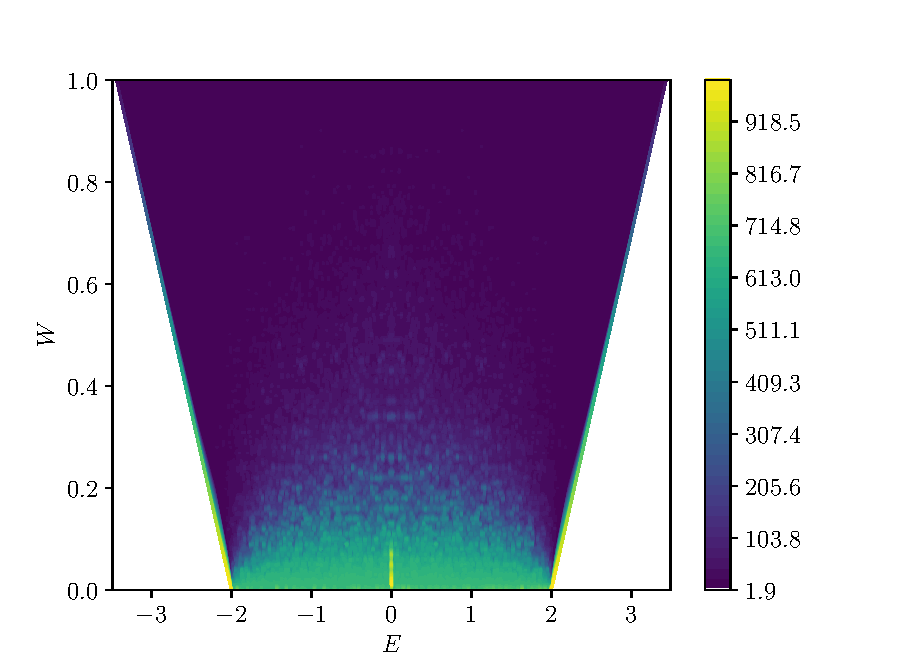
\includegraphics[width=\textwidth]{Figures/SSHIPR2.png}
\caption{IPR za primer, ko je nered v sklopitvah. Na vodoravni osi je energija stanj, na navpični pa jakost nereda $W$. Z barvo je označen IPR. Dolžina verige je 1000 mest.}
\label{fig:SSHIPR}
\end{figure}


\chapter{Model in metode dela}
Model, ki ga obravnavamo v tem delu, je nekoliko modificiran model SSH, opisan s Hamiltonjanom
\begin{equation} \label{spomnimo3}
\hat{H} = \sum_{n \in \mathbb{Z}} t_n \left( \frac{1}{2} \hat{c}_n^\dagger (\sigma_x + i \sigma_y) \hat{c}_{n+1} + \textup{h.c.} \right) + m_n \hat{c}_n^\dagger \sigma_y \hat{c}_n.
\end{equation}
Zaradi podobnosti z ostalimi deli na to temo \cite{mondragon} je notacija v tem razdelku drugačna kot v prej obdelanem modelu SSH, vendar lahko vseeno vidimo podobnosti: $t_n$ tukaj ustreza sklopitvi med različnimi osnovnimi celicami (prej $w$), medtem ko sklopitvi v osnovni celici (prej $v$) ustreza $\pm i m_n$. S $\hat{c}_n$ je označen vektor fermionskih operatorjev na obeh podmrežah, torej
$\hat{c}_n = (\hat{c}_{n,A} , \hat{c}_{n,B})^T$.
Zaradi prisotnosti imaginarne sklopitve v osnovni celici ta model za razliko od modela SSH nima simetrije na obrat časa ali simetrije na konjugacijo naboja, ima pa še vedno kiralno simetrijo. Formalno lahko topološke izolatorje klasificiramo na univerzalnostne razrede glede na njihove simetrije. V tej klasifikaciji spada model SSH v razred BDI, model (\ref{spomnimo3}) pa v razred AIII. Izkaže se \cite{mondragon}, da lahko vsak topološki izolator iz razreda AIII prevedemo na sistem nesklopljenih topoloških izolatorjev, opisanih z modelom (\ref{spomnimo3}). Zaradi te lastnosti bi dobro razumevanje fizike modela (\ref{spomnimo3}) privedlo do razumevanja fizike vseh topoloških izolatorjev v razredu AIII.
Operator kiralne simetrije za model (\ref{spomnimo3}) je enak:
\begin{equation}
\hat{\Gamma} = \sum_{n  \in \mathbb{Z}} \hat{c}_n^\dagger \sigma_3 \hat{c}_n.
\end{equation}
Nered bomo realizirali s pomočjo dveh naključno porazdeljenih spremenljivk - $\omega_n$ in $\omega_n^\prime$. Ti sta neodvisni in porazdeljeni po enakomerni porazdelitvi v intervalu $[ -0.5 , 0.5]$:
\begin{equation}
\omega_n, \omega_n^\prime \sim \mathcal{U}(-0.5,0.5).
\end{equation}
S temi nakjučnimi števili definiramo sklopitve na naslednji način:
\begin{align} \label{sklopitvi}
&t_n = 1 + 0.5 W \omega_n, \\
&m_n = m + W \omega_n^\prime. \label{sklopitvi2}
\end{align}
Nered je torej centriran okoli vrednosti $1$ oziroma $m$, njegovo jakost pa podaja število $W$.
Če nered ni prisoten, imamo kot v modelu SSH (poglavje \ref{spomnimoTIS}) na voljo dve topološki fazi, ki se ločita po ovojnem številu: $\nu=1$, če $m \in (-1,1)$ in $\nu=0$ sicer.

Ureditveni parameter v prisotnosti nereda bo še vedno ovojno število, vendar je njegov izračun tokrat nekoliko bolj zapleten.
Spomnimo se, da smo imeli v čistem sistemu na voljo formulo:
\begin{equation}
\nu = \frac{1}{2 \pi i} \int_0^{2 \pi} \frac{\partial \log h(k)}{\partial k} \textup{d}k = \frac{1}{2 \pi i} \int_0^{2 \pi} \frac{\partial h(k)}{\partial k} \frac{1}{h(k)} \textup{d}k,
\end{equation}
kjer je $h(k)$ naddiagonalna komponenta Hamiltonjana v recipročnem prostoru. V prisotnosti nereda nimamo več translacijske invariance in torej tudi nimamo več dobro določenega kristalnega valovnega vektorja. Očitno ta izraz za ovojno število ne bo uporaben, zato bomo zgornjo formulo zapisali v realnem prostoru.
To storimo z naslednjima substitucijama:
\begin{align}
&\frac{1}{2 \pi} \int_0^{2 \pi}\  \textup{d}k \to \frac{1}{N/2} \mathrm{Tr}, \\
&\frac{\partial}{\partial k} \to  -i [\hat{X}, \cdot ]. 
\end{align}
Prva formula predstavlja le zapis sledi na enoto volumna v krajevni bazi. Drugo formulo lahko izpeljemo na naslednji način: 
spomnimo se, da se v impulzni sliki operator položaja izraža kot $\hat{X} = i \frac{\partial}{\partial k}$. Potem lahko takoj izračunamo:
\begin{equation}
 -i [\hat{X}, f(k)] \psi(k) =  \frac{\partial \left(f(k) \psi(k) \right)}{\partial k} - f(k) \frac{\partial \psi(k)}{\partial k} = \frac{\partial f(k)}{\partial k} \psi(k),
\end{equation}
s čimer smo pokazali želeno zvezo.


Pred spremembo baze je bila v integrandu izvendiagonalna komponenta $h(k)$ Hamiltonjana v recipročnem prostoru. V realnem prostoru bo to sedaj matrika $\frac{N}{2} \times \frac{N}{2}$ - izvendiagonalni blok celotnega Hamiltonjana. Lažje bo računati s homotopsko ekvivalentnim Hamiltonjanom (spomnimo se, da homotopije ohranjajo ovojno število) $\hat{Q} = \hat{P}_+ -  \hat{P}_-$, kjer sta $\hat{P}_\pm$ projektorja na pozitivni oziroma negativni del spektra Hamiltonjana $\hat{H}$. Sedaj se spomnimo, da za operator kiralne simetrije $\hat{\Gamma}$ velja $\hat{\Gamma}^\dagger = \hat{\Gamma} $ in $\hat{\Gamma}^2 = \hat{\mathbb{I}}$, kar pomeni, da so njegove lastne vrednosti enake $\pm 1$. Zato ga lahko zapišemo kot $\hat{\Gamma} = \hat{\Gamma}_+ - \hat{\Gamma}_-$, kjer je operator $\hat{\Gamma}_+$ projektor na lastni podprostor, ki ustreza lastni vrednosti $1$, $\hat{\Gamma}_-$ pa na tisti, ki ustreza lastni vrednosti $-1$. Operatorja $\hat{\Gamma}_{+/-}$ sta popolnoma analogna operatorjema $\hat{P}_{A/B}$ v modelu SSH. Ker ima tudi Hamiltonjan $\hat{Q}$ kiralno simetrijo, ga lahko zapišemo kot
\begin{equation}
\hat{Q} = \hat{\Gamma}_+ \hat{Q} \hat{\Gamma}_- + \hat{\Gamma}_- \hat{Q} \hat{\Gamma}_+ = \hat{Q}_{+-} + \hat{Q}_{-+}.
\end{equation} 
Izvendiagonalni blok Hamiltonjana je potem preprosto $\hat{Q}_{+-}$, njegov inverz pa $\hat{Q}_{+-}^{-1} = \hat{Q}_{-+}$.
Sledi, da se formula za ovojno število glasi:
\begin{equation}
\nu = -\frac{1}{N/2} \mathrm{Tr} \left( \hat{Q}_{-+} [\hat{X},\hat{Q}_{+-}] \right).
\end{equation}
Zgornja formula velja, če računamo ovojno število za končno verigo z odprtimi robnimi pogoji. Če pa želimo izračunati ovojno število za sistem s periodičnimi robnimi pogoji, (kot ga bomo v nadaljevanju), se moramo v zgornji formuli znebiti operatorja $\hat{X}$, kajti  pri sistemih s takimi robnimi pogoji je ta slabo definiran.
V tem primeru izrazimo namesto substitucije $\partial_k \hat{Q}_{+-} \to -i [\hat{X}, \hat{Q}_{+-}]$ odvod po $k$ s končnimi diferencami \cite{diference}:
\begin{equation}
\partial_k \hat{Q}_{+-}(k) = \sum_m c_m \hat{Q}_{+-} (k+m \Delta ), 
\end{equation}
kjer so $c_m$ koeficienti končnih diferenc, najmanjša možna diferenca valovnega vektorja pa je enaka $\Delta  = \frac{4 \pi}{N}$, saj ima naš sistem $N/2$ osnovnih celic.
Odvisnosti od $k$ v operatorju $\hat{Q}_{+-}$ se lahko znebimo s pomočjo operatorja $e^{i k \hat{X}}$, ki predstavlja translacijo za moment $k$: 
\begin{equation}
\hat{Q}_{+-}(k+m \Delta ) =e ^{-i m \Delta  \hat{X}} \hat{Q}_{+-}(k) e^{i m \Delta  \hat{X}}.
\end{equation}
 Po prehodu v realni prostor dobimo formulo:
\begin{equation}
\nu = \frac{1}{N/2} \mathrm{Tr} (\sum_m c_m \hat{Q}_{-+} e^{-im \Delta \hat{X}} \hat{Q}_{+-} e^{im \Delta \hat{X}}).
\end{equation}
Iz formule za ovojno število sistema z odprtimi robnimi pogoji je razvidno, da je v limiti močnega nereda $W \to \infty$ ovojno število enako nič, saj v tem primeru vezi v osnovni celici dominirajo (to je razvidno iz enačb (\ref{sklopitvi}) in (\ref{sklopitvi2}) in je komutator $[\hat{X},\hat{Q}_{+-}]$ enak nič ($X$ označuje indeks osnovnih celic, ki so v tej limiti med sabo nesklopljene), medtem ko imamo po drugi strani pri $W=0$ in $m \in (-1,1)$ ovojno število enako ena, saj smo v tem primeru v topološki fazi modela SSH brez nereda. Ugotovili smo torej, da lahko med topološkimi fazami prehajamo tudi izključno s spreminjanjem jakosti nereda. Tak prehod je prikazan na sliki \ref{fig:InvariantVsW}, na kateri se vidi, da ovojno število pri točki faznega prehoda $W=4$ praktično takoj pade z $1$ na $0$. Na sliki je prikazan tudi rob energijskih pasov (valenčnega in prevodnega), kjer vidimo, da se ovojno število spremeni šele daleč po tem, ko se energijska reža zapre, kar se zgodi že pri $W=3$.
\begin{figure}[!h]
\centering
\begin{subfigure}{.7\textwidth}
\includegraphics[width=\linewidth]{Figures/InvariantVsW2.png}
\end{subfigure}
\caption{ovojno število v odvisnosti od jakosti nereda pri $m=0$. Rezultati so povprečeni po $200$ realizacijah nereda. Opazimo nenadno spremembo pri približno $W=4$, medtem ko se energijska reža zapre pri $W=3$. Vir slike: \cite{mondragon}.}
\label{fig:InvariantVsW}
\end{figure}

Izkaže se, da kritična črta (množica vseh kritičnih točk) sovpada s točkami divergence lokalizacijske dolžine stanja z ničelno energijo. Zaradi Andersonove lokalizacije so stanja v prisotnosti nereda lokalizirana, v kritični točki pa se pojavi delokalizirano stanje pri energiji nič.
To se da videti iz eksplicitne rešitve Schrödingerjeve enačbe z ničelno energijo. Označimo to rešitev z $|  \Psi \rangle$.
To stanje lahko zapišemo kot:
\begin{equation}
| \Psi \rangle = \sum_{\substack{n \in \mathbb{Z} \\ \alpha \in \{ \textup{A,B}\}}} \Psi_{n, \alpha} |n, \alpha \rangle,
\end{equation}
kjer $n$ označuje indeks osnovne celice.
Schrödingerjeva enačba se glasi:
\begin{align}
&H \Psi = 0, \\
& t_{n-1} \Psi_{n-1,\textup{A}} + i m_n \Psi_{n,\textup{A}} = 0,\\
&t_n \Psi_{n+1, \textup{B}} -  i m_n \Psi_{n, \textup{B}} = 0.
\end{align}
Iz zgornje enačbe lahko rekurzivno izrazimo rešitev:
\begin{equation}
\Psi_{n+1, \textup{B}} = i^n \left( \prod_{j=1}^n \frac{m_j}{t_j} \right) \Psi_{1,\textup{B}}
\end{equation}
in podobno za $\Psi_{n,\textup{A}}$.
Za velike $n$ definirajmo $|\Psi_{n, \textup{B}}| = e^{-n/\Lambda } |\Psi_{1, \textup{B}}|$. Z $\Lambda$ smo označili lokalizacijsko dolžino stanja.
Iz zgornje rekurzivne enačbe dobimo izraz zanjo:
\begin{equation}
\Lambda^{-1} = \left| - \lim_{n \to \infty} \frac{1}{n} \log |\Psi_{n, \textup{B}}| / |\Psi_{1, \textup{B}}| \right|.
\end{equation}
Če vstavimo rekurzivni izraz za $\Psi_{n, \textup{B}}$, dobimo:
\begin{equation} \label{empiricnalok}
\Lambda^{-1} = \left| \lim_{n \to \infty} \frac{1}{n} \sum_{j=1}^n ( \log |m_j| - \log |t_j| ) \right|.
\end{equation}
Zgornjo formulo bi radi poenostavili. 
To lahko naredimo s pomočjo Birkhoffovega ergodičnega izreka \cite{birkhoff}.
\begin{theorem*}
Naj bo $X$ stacionaren in ergodičen stohastični proces in $f$ takšna funkcija, da velja $E(|f|) < \infty$. Potem velja:
\begin{equation}
\lim_{n \to \infty} \frac{1}{n} \sum_{j=1}^{n} f(\theta_j X) = E(f(X)),
\end{equation}
kjer je $\theta_j (x_1,x_2,x_3, \dots) = (x_j,x_{j+1},x_{j+2}, \dots)$ operator premika za $j-1$ mest, $E(f)$ pa označuje pričakovano vrednost $f$.
\end{theorem*}
V našem primeru predstavlja stohastični proces $X$ vzorce naključnih spremenljivk $X=((t_1,m_1),(t_2,m_2),(t_3,m_3), \dots)$. Ta proces je stacionaren in ergodičen, saj so posamezni vzorci neodvisni in enako porazdeljeni \cite{birkhoff} (izrek lahko sicer uporabimo tudi v splošnejših primerih, ko so vzorci na primer paroma korelirani).
Funkcija $f$ je v našem primeru enaka  $f((t_1,m_1),( t_2, m_2), ...) = \log |m_1| - \log |t_1|$.
Izrazimo sklopitve $t_n$ in $m_n$ s formulama (\ref{sklopitvi}) in izračunajmo pričakovano vrednost $|f|$:
\begin{equation}
E(|f|) = \int_{-0.5}^{0.5} \textup{d} \omega \int_{-0.5}^{0.5} \textup{d} \omega^\prime \left| \log | m + W_2 \omega | - \log | 1 + W_1 \omega^\prime | \right|.
\end{equation}
Ker integriramo po končnem intervalu, je morebiten problematičen del le tisti, kjer ima logaritem divergenco, na primer, ko velja $\omega \sim -\frac{1}{W_2}$. Ko primerno razbijemo integral na manjše intervale in se znebimo absolutne vrednosti v integrandu, dobi tak problematičen del obliko $\lim_{\epsilon \to 0} \int_{- \epsilon}^\epsilon \log |x| dx =  2 \lim_{\epsilon \to 0} \int_{0}^\epsilon \log x dx = \lim_{\epsilon \to 0} x (\log x - 1) \rvert_0^\epsilon = 0$. Del blizu divergence torej k integralu ne prispeva in velja $E(|f|) < \infty$.

Sedaj lahko direktno uporabimo Birkhoffov izrek, da dobimo
\begin{equation}
\Lambda^{-1} = \left| \int_{-0.5}^{0.5} \textup{d} \omega \int_{-0.5}^{0.5} \textup{d} \omega^\prime ( \log | m + W_2 \omega | - \log | 1 + W_1 \omega^\prime | ) \right|,
\end{equation}
kar se da analitično izračunati \cite{mondragon}. Rezultat je:
\begin{equation} \label{analiticnalok}
\Lambda^{-1} = \left| \log( \frac{|2+W_1|^{1/W_1 + 0.5} |2m - W_2|^{m/W_2 -0.5}}{|2-W_1|^{1/W_1-0.5} |2m + W_2|^{m/W_2 + 0.5}})\right|.
\end{equation}

\begin{figure}[!h]
\centering
\begin{subfigure}{.7\textwidth}
\includegraphics[width=\linewidth]{Figures/CriticalSurface.png}
\end{subfigure}
\caption{na levi je prikazan fazni diagram modela (\ref{spomnimo3}). Na desni je prikazana lokalizacijska dolžina stanja z $E=0$, ki divergira na kritični črti. Prav tako je na desni z zeleno črto označena pot, po kateri bomo pozneje izvedli preklop Hamiltonjana. Izračuni za $\nu$ so narejeni na verigi velikosti $N=2000$ in povprečeni preko $10$ realizacij nereda. Vir slike: \cite{mondragon}.}
\label{fig:CriticalSurface}
\end{figure}

Na sliki \ref{fig:CriticalSurface} je prikazan fazni diagram obravnavanega modela. Opazimo, da divergenca lokalizacijske dolžine pri ničelni energiji res sovpada s kritično črto. Kot prej povedano, lahko poleg prehajanja med fazama, ki smo ga videli že v modelu SSH, preidemo iz topološke v trivialno fazo tudi z dovolj močno jakostjo nereda. Zanimali nas bodo preklopi Hamiltonjana čez fazni prehod, kjer bomo povečevali $W$ pri $m=0$, kot je na desnem grafu označeno z zeleno črto.
Zaenkrat nekaj o tem faznem prehodu že vemo: če razvijemo enačbo (\ref{analiticnalok}) okoli $W_C=4$, pri $m=0$, vidimo, da lokalizacijska dolžina v bližini faznega prehoda skalira kot $\Lambda \sim \frac{1}{|W-W_C| \log |W-W_C|}$. Kritični eksponent, ki opisuje skaliranje lokalizacijske dolžine za obravnavani fazni prehod, je torej enak ena z logaritemskim popravkom.

Oglejmo si obnašanje modela vzdolž poti, preko katere bomo izvedli preklop. 
Kot prvi test in občutek za potrebno velikost verige $N$ si poglejmo primerjavo empirične (\ref{empiricnalok}) in analitične (\ref{analiticnalok}) formule za lokalizacijsko dolžino vzdolž te poti za več velikosti sistema.
\begin{figure}[!h]
\centering
\begin{subfigure}{.9\textwidth}
\includegraphics[width=\linewidth]{Figures/locLength.pdf}
\end{subfigure}
\caption{inverz lokalizacijske dolžine, pridobljen z empirično formulo za več velikosti sistema ($N$ prikazuje število vseh atomov v verigi) in z analitično formulo za neskončno dolgo verigo vzdolž poti $W: 3 \to 5$ pri $m=0$.}
\label{fig:locLength}
\end{figure}
Na sliki \ref{fig:locLength} vidimo, da za velikosti verige nekaj tisoč atomov še ne pridemo do točnega asimptotskega obnašanja - za to potrebujemo verigo dolžine več sto tisoč atomov -, vendar je obnašanje lokalizacijske dolžine pri tako majhnih verigah vseeno kvalitativno zelo podobno obnašanju neskončne verige. V nadaljevanju bomo (če ne bo drugače rečeno) obravnavali verigo z $N=1000$. Za večje $N$ postanejo numerične metode, ki jih bomo uporabljali, časovno prezahtevne. Vse izračune, ki sledijo, smo ponovili za dvakrat daljšo verigo, kjer ni bilo opaziti bistvenih razlik. Na sliki lahko opazimo še naslednje: ko imamo opravka z končno verigo, se divergenca lokalizacijske dolžine (in s tem fazni prehod) ne pojavi točno pri $W_C=4$, kot narekuje asimptotska formula, temveč v bližini te točke. Izkaže se, da to ni problem, saj bomo pri ekscitacijah rezultate tako ali tako povprečevali po dovolj veliko realizacijah nereda, da lahko privzamemo, da je povprečna kritična točka res $W_C=4$.

Sedaj si poglejmo, kako izgledajo energijski nivoji Hamiltonjana modela (\ref{spomnimo3}) vzdolž prej omenjene poti čez fazni prehod. 
V ta namen napišimo Hamiltonjan v matrični obliki:
\[
H = \begin{bmatrix} 
0 & i m_1 &  &  &  & t_{N/2}\\
-i m_1 & 0 & t_1 &  & &  \\
 & t_1 & 0 & im_2 &  &  \\
 &  & -im_2 & 0& \ddots&  & \\
 &  &  & \ddots & \ddots & im_{N/2}  \\
t_{N/2} & & &  & -i m_{N/2} & 0  
    \end{bmatrix}
\]
Izbrali smo periodične robne pogoje, saj nas bo zanimala fizika v notranjosti. Energije bomo dobili z diagonalizacijo zgornje matrike.
Iz spektra lahko izračunamo tudi gostoto stanj. Formalno je to vsota Diracovih funkcij delta pri lastnih energijah:
\begin{equation}
g(E) = \sum_{i=1}^N \delta (E_i - E).
\end{equation}
Za potrebe prikaza smo Diracove funkcije delta aproksimirali z Lorentzovo krivuljo:
\begin{equation}
\delta (x) = \lim_{\sigma \to 0} \frac{1}{\pi} \frac{\sigma}{\sigma^2 + x^2}.
\end{equation}
V izračunih smo vzeli vrednost $\sigma=0.01$.
Rezultati, ki jih da numerika, so sledeči:
\begin{figure}[!h]
\centering
\begin{subfigure}{\textwidth}
\includegraphics[width=\linewidth]{Figures/Nicegraph1.pdf}
\end{subfigure}
\caption{prikazanih je nekaj najnižjih lastnih energijskih nivojev vzdolž poti $W: 2 \to 6$ pri $m=0$. Na spodnjih treh grafih je za različna mesta vzdolž poti prikazana gostota stanj.}
\label{fig:Nicegraph1}
\end{figure}
Na sliki \ref{fig:Nicegraph1} vidimo nekaj najnižjih pozitivnih energijskih nivojev vzdolž poti, preko katere bomo izvajali preklop. Slika za negativne energije je enaka, saj je zaradi kiralne simetrije spekter simetričen. Opazimo, da se pri približevanju kritični točki energijska reža res zapira in ostane tudi po prehodu skozi kritično točko $W_C=4$ zaprta. Na spodnjih treh grafih je prikazana gostota stanj, pridobljena za tri točke vzdolž poti. Prva ustreza $W=2.5$, kar je še daleč od kritične točke, in kjer je energijska reža še odprta, kar vidimo v ničelni gostoti stanj okoli energije nič. Okoli $W=3.5$ je energijska reža že zaprta, kar lahko potrdimo s tem, da je gostota stanj pri $E=0$ neničelna. V kritični točki je v gostoti stanj divergenca pri energiji $0$. Podobno obnašanje gostote stanj opazimo tudi pri večjih sistemih, kjer ugotovimo, da je gostota stanj pri energiji nič neničelna, če velja $W\geq 3$. $W=3$ je torej točka, v kateri se energijska reža zapre.
\begin{figure}[!h]
\centering
\begin{subfigure}{\textwidth}
\includegraphics[width=\linewidth]{Figures/Nicegraph2.pdf}
\end{subfigure}
\caption{prikazanih je nekaj najnižjih lastnih energijskih nivojev v logaritemski skali vzdolž poti $W: 2 \to 6$ pri $m=0$. S črtkano črno črto je označena lokalizacijska dolžina stanja z energijo nič, pridobljena s formulo \ref{empiricnalok}. Pripadajoča skala je na desni strani.}
\label{fig:Nicegraph2}
\end{figure}
Na sliki \ref{fig:Nicegraph2} so energijski nivoji prikazani v logaritemski skali. Tu se nazorneje vidi, da pride pogosto do odboja nivojev, kot je na primer razvidno na povečanem delu grafa.
Na grafu je prikazana tudi lokalizacijska dolžina stanja z energijo nič in vidimo lahko, da se v točki, kjer ta divergira, energijski nivoji najbolj približajo ničli. To je povezano z že prej opaženo divergenco gostote stanj pri $E=0$, ki je najmočnejša v kritični točki. 
Opazimo lahko, da če v formuli (\ref{sklopitvi}) za sklopitvi $t_n$ in $m_n$ vstavimo $W_C=4$,  sta velikosti obeh sklopitev v povprečju enaki, kar pomeni, da bi lahko veljala formula, izpeljana v dodatku B: $g(E) \propto \frac{-1}{|E| \log^3 |E|}$.
Poglejmo si, kaj točno se zgodi z gostoto stanj v našem primeru. Izračunali smo histogram lastnih energij sistema velikosti $N=10000$ z odprtimi robnimi pogoji za $10000$ realizacij nereda. Histogram, katerega vrednosti so sorazmerne z gostoto stanj, smo prilagodili funkciji $g(E) \propto \frac{-1}{|E|^{1+x} \log^y |E|}$. Rezultati so prikazani na sliki \ref{fig:dos}, kjer rišemo logaritem funkcije $E*g(E)$ v odvisnosti od logaritma energije. Opazimo, da je divergenca gostote stanj res najmočnejša v kritični točki, kar se ujema s sliko \ref{fig:Nicegraph2}. V kritični točki velja $x \approx 10^{-4}, y \approx 3.03$, kar je v zelo dobrem ujemanju z izpeljano formulo. Zunaj kritične točke, pri $W=3.9$, potenca na logaritmu hitro pade. Ko se od kritične točke še oddaljujemo, pa postane vrednost parametra $x$ znatna in negativna in dodatno ublaži divergenco.
\begin{figure}[!h]
\centering
\begin{subfigure}{.9\textwidth}
\includegraphics[width=\linewidth]{Figures/DOSHist.pdf}
\end{subfigure}
\caption{prikaz skaliranja gostote stanj v okolici $E=0$ za tri različne vrednosti parametra $W$. Rezultati so pridobljeni za sistem velikosti $N=10000$ z odprtimi robnimi pogoji in povprečeni preko $10000$ realizacij nereda.}
\label{fig:dos}
\end{figure} \newpage
Na sliki \ref{fig:SSHIPRNered} je prikazan IPR za model, ki ga obravnavamo. Tu je že v čistem modelu IPR majhen, saj čisti model ustreza eni izmed popolnoma dimeriziranih limit v modelu SSH (poglavje \ref{spomnimoRobna}). Ko dodamo nered, ostanejo stanja močno lokalizirana. Tudi v okolici točke $W_C=4, E=0$ ni videti nobene delokalizacije, kar se zdi v nasprotju z našo prejšnjo izpeljavo. Izkaže se \cite{mondragon}, da delokalizirano stanje nastane kot linearna kombinacija velikega števila degeneriranih lokaliziranih stanj z energijo nič. Teh je v neskončno velikem sistemu veliko, kar se vidi v divergenci gostote stanj okoli energije nič, v končnem sistemu pa imamo takšnih nizkoenergijskih stanj malo. V praksi zato delokaliziranega stanja ne bomo opazili.
\begin{figure}[!h]
\centering
\begin{subfigure}{.6\textwidth}
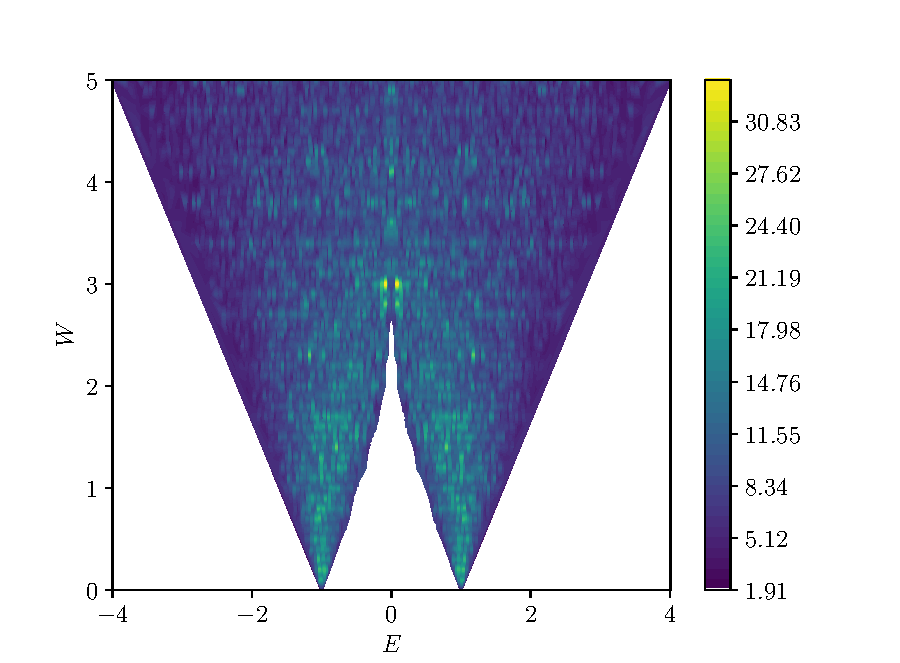
\includegraphics[width=\linewidth]{Figures/SSHIPRNered.pdf}
\end{subfigure}
\caption{IPR v odvisnosti od jakosti nereda $W$ in energije $E$.}
\label{fig:SSHIPRNered}
\end{figure} \newpage
Na sliki \ref{fig:EigenPloti} so prikazane nekatere lastne funkcije modela pred kritično točko in v njej. Opazimo, da so vse lokalizirane, čeprav se v kritični točki že vidi drugačno obnašanje stanja z najnižjo energijo. To ima, za razliko od ostalih, posamezna vrhova precej daleč narazen. Na grafu sicer izgleda, da ima tudi stanje pri $W=3.8$ močno razmaknjena vrhova, toda v resnici sta ta vrhova blizu, saj so robni pogoji periodični.
\begin{figure}[!h]
\centering
\begin{subfigure}{.7\textwidth}
\includegraphics[width=\linewidth]{Figures/EigenPloti.pdf}
\end{subfigure}
\caption{na levi so prikazane prve 3 lastne funkcije s pozitivno energijo pri $W=3.8$, na desni pa pri $W=4$.}
\label{fig:EigenPloti}
\end{figure}

Sedaj se bomo posvetili preklopom Hamiltonjana čez fazni prehod, kar pomeni, da bomo spremljali časovni razvoj valovne funkcije, pri čemer bomo parametre Hamiltonjana spreminjali linearno s časom vzdolž prej omenjene poti.
Preklop med dvema vrednostima jakosti nareda delamo tako, da začnemo pri vrednosti $W_{\textup{z}}<4$, končamo pa, po določenem času preklopa $T$, pri vrednosti $W_{\textup{k}}>4$.
Časovno odvisnost jakosti nereda lahko torej zapišemo kot: 
\begin{equation}
W(t) = W_{\textup{z}} +  t/T (W_{\textup{k}}-W_{\textup{z}}).
\end{equation} 
Začnemo v lastnem enodelčnem stanju $\Psi(t=0)$ iz valenčnega pasu pri $W_{\textup{z}}$ in ga časovno razvijemo. Ker delamo preklop, je tudi Hamiltonjan odvisen od časa.
Rešujemo torej časovno odvisno Schrödingerjevo enačbo:
\begin{equation}
i \frac{\partial \Psi (t)}{\partial t} = \hat{H}(t) \Psi(t).
\end{equation}
Rešitev izrazimo s pomočjo operatorja časovnega razvoja $\hat{U}(t, \tau) = e^{-i \hat{H}(t) \tau}$ kot $\Psi(t+\tau) \approx \hat{U}(t,\tau) \Psi(t)$.
Ta shema bo delovala, če je časovni korak $\tau$ dovolj majhen, da lahko v intervalu $[t, t+\tau]$ privzamemo, da je Hamiltonjan konstanten in enak $H(t)$. Za numeričen izračun časovnega razvoja bomo uporabili implicitno metodo tipa Crank-Nicholson, ki zagotavlja, da je operator časovnega razvoja unitaren.
Uporabili bomo Padéjevo aproksimacijo za eksponentno funkcijo:
\begin{equation}
\exp (-i \tau \hat{H}) = \left(\hat{\mathbb{I}} + i \frac{\tau}{2} \hat{H} \right)^{-1}   \left(\hat{\mathbb{I}} - i \frac{\tau}{2} \hat{H} \right) + \mathcal{O}(\tau^3),
\end{equation} 
s čimer dobimo implicitno shemo:
\begin{equation}
\left( \hat{\mathbb{I}} + i \frac{\tau}{2} \hat{H}(t) \right) \Psi (t+\tau) = \left(\hat{\mathbb{I}}- i \frac{\tau}{2} \hat{H}(t) \right) \Psi(t).
\end{equation}
Pogosto bomo časovno razvijali več funkcij hkrati. To bi lahko storili tako, da bi zgornjo enačbo reševali za vsako izmed njih, a je učinkoviteje, če rešujemo matrično enačbo:
\begin{equation}
\left( \mathbb{I} + i \frac{\tau}{2} \hat{H}(t) \right) X(t+\tau) = \left(\mathbb{I}- i \frac{\tau}{2} \hat{H}(t) \right) X,
\end{equation}
kjer so v matriki $X$ lastni vektorji $\Psi$ v stolpcih.
V našem primeru bomo vzeli vrednost $\tau=1$. Takšna izbira se zdi smiselna, saj smo videli, da je veliko lastnih energij reda velikosti krepko pod $1$, kar ustreza relevantni časovni skali veliko več kot $1$. Rezultate smo preverili tudi pri $\tau=0.5$, kjer nismo opazili razlike.

Med preklopom se pojavijo ekscitacije v prevodnem pasu, saj je čas preklopa končen.
Število ekscitacij v i-to lastno stanje oziroma zasedenost i-tega lastnega stanja izračunamo preprosto kot
\begin{equation}
N_i = \sum_j |\langle i | \Psi_j \rangle|^2,
\end{equation}
kjer je $\Psi_j$ časovno razvito j-to stanje iz valenčnega pasu, $| i \rangle$ pa predstavlja i-to lastno stanje Hamiltonjana ob nekem času. Vrednost $| \langle i | \Psi_j \rangle |^2$ je verjetnost, da med preklopom elektron iz začetnega stanja j-tega lastnega stanja preskoči v lastno stanje $| i \rangle$. Celotno verjetnost za prehod v stanje $| i \rangle$ in s tem zasedenost tega stanja potem dobimo tako, da to seštejemo po vseh časovno razvitih stanjih iz valenčnega pasu $\Psi_j$.

Pri obravnavi ekscitacij bomo iskali odvisnosti oblike 
\begin{equation}
N_{\textup{eks}} = \alpha T^{\beta} \log^\gamma T,
\end{equation}
kjer $N_{\textup{eks}}$ označuje celotno število ekscitacij v prevodnem pasu. Zanimala nas bosta predvsem potenci $\beta$ in $\gamma$. Za pridobitev le-teh iz podatkov zgornjo enačbo najprej logaritmiramo
\begin{equation}
\log N_{\textup{eks}} = \log \alpha + \beta \log T + \gamma \log \log T.
\end{equation}
Z definicijami $z=\log N_{\textup{eks}}$, $x=\log T$ in $y=\log \log T$ tako dobimo linearno funkcijo $z=\log \alpha + \beta x + \gamma y$, ki jo lahko preprosto prilagajamo podatkom.

\chapter{Rezultati}
Poglejmo, kolikšno je število ekscitacij po preklopu za več časov trajanja preklopa. Preklop bomo delali za različno dolge intervale jakosti nereda $[W_{\textup{z}}, W_{\textup{k}}]$, pri čemer bo vedno veljalo, da je kritična točka $W_C=4$ na sredini tega intervala. Na levem grafu slike \ref{fig:Skaliranje} se vidi, da število ekscitacij pada s časom trajanja preklopa, kar je smiselno, saj vemo, da adiabatski preklop, v katerem se ekscitacije ne pojavijo, ustreza neskončno dolgem preklopu.
Prav tako opazimo, da imamo več ekscitacij, če preklapljamo na daljšem intervalu jakosti nereda $[W_{\textup{z}}, W_{\textup{k}}]$. To se zgodi, ker pri najkrajšem intervalu ne preklapljamo dovolj počasi in število ekscitacij še ne saturira, kot bo vidno na sliki \ref{fig:SkoziCas}. Odvisnost števila končnih ekscitacij od časa trajanja preklopa dobro opiše potenčni zakon z logaritemskim popravkom. Potence so sicer odvisne od intervala jakosti nereda, preko katerega izvajamo preklop, vendar lahko na grafu opazimo, da smo pri preklopoma na daljšem intervalu jakosti nereda že blizu nekakšnem limitnem obnašanju. 
\begin{figure}[!h]
\centering
\begin{subfigure}{.99\textwidth}
\includegraphics[width=\linewidth]{Figures/Skaliranje3Alt.pdf}
\end{subfigure}
\caption{na levi je prikazano število vseh ekscitacij po koncu preklopa v odvisnosti od njegovega časa trajanja $T$, na desni pa v odvisnosti od njegove hitrosti $v$. Podatki so prikazani za 3 različne izbire $W_{\textup{z}}$ in $W_{\textup{k}}$.}
\label{fig:Skaliranje}
\end{figure}
Pravzaprav je smiselneje gledati število ekscitacij v odvisnosti od hitrosti preklopa $v=(W_{\textup{k}}-W_{\textup{z}})/T$ (namreč, preklop $W \in [3.5, 4.5]$ pri $T=10000$ je enako hiter kot preklop $W \in [2,6]$ pri $T=40000$), kar je prikazano na desnem grafu slike \ref{fig:Skaliranje}. Tu bolje opazimo, da sta si preklopa na daljšem intervalu veliko bolj podobna v obnašanju - v primerjavi s preklopom na krajšem. 
\begin{figure}[!h]
\centering
\begin{subfigure}{.99\textwidth}
\includegraphics[width=\linewidth]{Figures/SkoziCas.pdf}
\end{subfigure}
\caption{skupno število ekscitacij med preklopom, prikazano za več različnih intervalov preklopa in hitrosti preklopa.}
\label{fig:SkoziCas}
\end{figure}
Na sliki \ref{fig:SkoziCas} opazimo prej omenjeno saturacijo števila ekscitacij po koncu preklopa pri širšem intervalu preklopa ter pri počasnih preklopih.
Podobno kot v energijskih nivojih se pojavi asimetrija območja pred kritično točko $W_C=4$ in po njem.
Sedaj bomo osi na sliki \ref{fig:SkoziCas} reskalirali. Uvedimo količini $\tilde{N}_{\textup{eks}}(t) = N_{\textup{eks}}(t)/N_{\textup{eks}}(T)$ in $\tilde{W} = (W-W_C)T^x (\log T)^y+W_C$, kjer sta $x, y$ skalirna eksponenta $N_{\textup{eks}} \propto T^{-x} (\log T)^{-y}$. Na sliki \ref{fig:SkoziCasAlt} je narisana odvisnost $\tilde{N}_{\textup{eks}}$ od $\tilde{W}$. Vidimo, da je obnašanje teh krivulj univerzalno za več različnih preklopov. Najhitrejši preklopi odstopajo od tega obnašanja, vendar smo to pričakovali, saj smo že povedali, da spadajo ti v drugačen režim, v katerem število ekscitacij še ni saturiralo.
\begin{figure}[!h]
\centering
\begin{subfigure}{.99\textwidth}
\includegraphics[width=\linewidth]{Figures/SkoziCasAlt.pdf}
\end{subfigure}
\caption{skupno število ekscitacij med preklopom, prikazano za več različnih intervalov preklopa in hitrosti preklopa. Vsak graf je reskaliran s primernimi potencami, pridobljenimi iz slike \ref{fig:Skaliranje}.}
\label{fig:SkoziCasAlt}
\end{figure}
Poglejmo si še, kje natančneje se pojavijo te ekscitacije. Na sliki \ref{fig:Krajevne} je prikazana krajevna porazdelitev ekscitacij med preklopom. Vidimo, da se ekscitacije pojavijo na naključnih osnovnih celicah, katerih zasedenost potem s časom še raste.
\begin{figure}[!h]
\centering
\begin{subfigure}{.99\textwidth}
\includegraphics[width=\linewidth]{Figures/KrajevneEksitacijeNoGrid.pdf}
\end{subfigure}
\caption{na sliki so porazdelitve ekscitacij po osnovnih celicah na verigi s $500$ osnovnimi celicami, ki traja $T=6000$ in poteka na intervalu $W \in [3,5]$.}
\label{fig:Krajevne}
\end{figure}
\newpage
Poglejmo si še porazdelitev ekscitacij po lastnih stanjih Hamiltonjana. To je prikazano na sliki \ref{fig:EksTekom} za dve realizaciji nereda. Kot smo že videli (slika \ref{fig:SkoziCas}), se posamezne ekscitacije začnejo pojavljati že nekaj pred kritično točko, njihovo število se pri prehodu kritične točke poveča, za kritično točko pa saturira in nimamo več novih ekscitacij. 

\begin{figure}[!h]
\centering
\begin{subfigure}{.49\textwidth}
\includegraphics[width=\linewidth]{Figures/EksTekom1.pdf}
\end{subfigure}
\begin{subfigure}{.49\textwidth}
\includegraphics[width=\linewidth]{Figures/EksTekom2.pdf}
\end{subfigure}
\caption{energijski nivoji deset najnižjih stanj v prevodnem pasu in ekscitacije za dve realizaciji nereda. Število ekscitacij predstavljata velikost in barva pikic. Hitrost preklopa je $v=0.01$, preklapljamo pa na intervalu $W \in [3,5]$.}
\label{fig:EksTekom}
\end{figure} \newpage
Na sliki \ref{fig:EksBini2} smo interval energij $E \in [10^{-13},1]$ v logaritemski skali razdelili na 50 enako velikih območij in opazovali ekscitacije, ki padejo vanje, povprečene preko $100$ realizacij nereda. Prikazana sta grafa za dve različni hitrosti preklopa. Opazimo, da imajo po počasnejšem preklopu (na desni sliki) najvišje vzbujeni elektroni manjšo energijo, kot po hitrejšem (na levi sliki). Tudi to bi lahko pričakovali, saj že vemo, da je nasploh več ekscitacij v hitrejših preklopih.
\begin{figure}[!h]
\centering
\begin{subfigure}{.49\textwidth}
\includegraphics[width=\linewidth]{Figures/EksBini3.pdf}
\end{subfigure}
\begin{subfigure}{.49\textwidth}
\includegraphics[width=\linewidth]{Figures/EksBini4.pdf}
\end{subfigure}
\caption{število ekscitacij na interval energije med preklopom. Interval $E \in [10^{-13},1]$ smo razdelili na 50 enako velikih delov v logaritemski skali in narisali število ekscitacij na vsak interval, povprečeno po $100$ realizacijah nereda. Levi graf je za $v=0.001$, desni pa za $v=0.0001$.}
\label{fig:EksBini2}
\end{figure}
\newpage
Na sliki \ref{fig:Emax} si podrobneje ogledamo, kako je z ravnokar omenjeno odvisnostjo energij, do katerih so stanja zasedena od hitrosti preklopa. Opazujemo, pri kateri energiji $E_{\textup{max}}$ pade zasedenost stanj s $0.5$ na $0.25$, kar služi kot ocena za robno energijo, nad katero ni več veliko ekscitacij. Če to narišemo v odvisnosti od hitrosti preklopa, opazimo, da je odvisnost približno korenska.
\begin{figure}[!h]
\centering
\begin{subfigure}{.9\textwidth}
\includegraphics[width=\linewidth]{Figures/Emax.pdf}
\end{subfigure}
\caption{na grafu je prikazana energija najvišje zasedenih stanj po koncu preklopa za več njegovih hitrosti. To je energija, kjer število ekscitacij prvič pade na $0.25$. Rezultati so povprečeni po $100$ realizacijah nereda, energijski interval $E \in [10^{-13},1]$ pa smo razdelili na $300$ delov. Preklop je potekal na intervalu $W \in [3,5]$.}
\label{fig:Emax}
\end{figure}
\newpage
Na sliki \ref{fig:IzEngaStanja} lahko vidimo, v katera stanja prehaja elektron, ki je na začetku v  stanju na zgornjem robu valenčnega pasu. Obnašanje je podobno pri ostalih stanjih blizu zgornjega roba. Opazimo, da preidemo po kritični točki z verjetnostjo približno $0.5$ v prevodni pas, v katerem imamo praviloma na voljo dve stanji, v kateri lahko preidemo z verjetnostjo $0.25$. Ti stanji, v kateri lahko skočimo, sta ravno kiralna partnerja (poglavje \ref{spomnimo4}) stanj, v katerih ostanemo, če ne pride do skoka v prevodni pas.  
\begin{figure}[!h]
\centering
\begin{subfigure}{.9\textwidth}
\includegraphics[width=\linewidth]{Figures/IzEngaStanja.pdf}
\end{subfigure}
\caption{na grafu je z barvo prikazana verjetnost za prehod v različna lastna stanja Hamiltonjana med preklopom, če preklapljamo lastno stanje, ki ima na začetku najvišjo negativno energijo (torej prvo stanje v valenčnem pasu). Zgornji graf prikazuje prevodni pas, spodnji pa valenčnega. Na grafu so označena tudi zaporedna števila stanj, v katera prehajamo. Stanje z zaporedno številko $1$ je na spodnjem robu prevodnega oziroma na zgornjem robu valenčnega pasu, zaporedno število stanj pa potem od roba proti notranjosti narašča.}
\label{fig:IzEngaStanja}
\end{figure}
\newpage
Opazili smo, da se po prehodu skozi kritično točko lahko indeksi zasedenih stanj še nadalje spreminjajo. Razlago za to lahko vidimo na sliki \ref{fig:IzEngaStanjaWBand}. Po prehodu ostanejo energijski nivoji tesno blizu, kar pomeni, da lahko elektron še nadalje skoči na naslednji energijski nivo.

\begin{figure}[!h]
\centering
\begin{subfigure}{.9\textwidth}
\includegraphics[width=\linewidth]{Figures/IzEngaStanjaWBand.pdf}
\end{subfigure}
\caption{na grafu je nekaj najnižjih energijskih nivojev v prevodnem pasu. S pikicami so označene verjetnosti za prehod v prevodni pas, če preklapljamo stanje z najvišjo energijo v valenčnem pasu.}
\label{fig:IzEngaStanjaWBand}
\end{figure}

%\input{Zaklju"cek}
\chapter{Zaklju"cek}
Obravnavali smo počasne preklope Hamiltonjana v prirejenem modelu SSH. Ta opiše enodimenzionalen topološki izolator z dvema topološkima fazama, ki se razlikujeta po topološki invarianti -  ovojnem številu. V sklopitve smo dodali nered, kar povzroči, da se lastna stanja lokalizirajo. Opazili smo, da lahko med fazama prehajamo tudi izključno z večanjem jakosti nereda in se najprej osredotočili na lastnosti takšnega faznega prehoda. Na širšem območju okoli kritične točke je energijska reža zaprta, točno v kritični točki pa se pojavi delokalizirano lastno stanje pri energiji nič.  
Začenši v topološki fazi smo izvajali preklop preko te kritične točke in opazovali ekscitacije v prevodnem pasu, ki se pri tem pojavijo. Ugotovili smo, da za počasne preklope število teh skalira potenčno s hitrostjo preklopa z logaritemskim popravkom, kjer so potence odvisne od intervala jakosti nereda, preko katerega izvajamo preklop. Opazili smo, da to obnašanje z daljšanjem intervala jakosti nereda konvergira k nekem limitnem obnašanju.
Če reskaliramo čas s pridobljenimi potencami, opazimo pri počasnih preklopih univerzalno obnašanje odvisnosti števila ekscitacij s časom tekom preklopa.
Potenčni zakon se pojavi tudi pri skaliranju energij najvišje zasedenih elektronskih ekscitacij po koncu preklopa, kjer smo opazili približno korensko odvisnost od hitrosti preklopa.
Videli smo, da v kritični točki časovno razvito stanje iz valenčnega pasu praviloma preide v le dve različni stanji v prevodnem pasu z enako verjetnostjo ali pa ostane v valenčnem pasu v kiralnem partnerju enega izmed teh dveh stanj.  Podrobnejšega razumevanja teh prehodov še nimamo, zato bi bilo idealno nadaljevanje našega dela raziskovanje v tej smeri. Nove pristope k analizi obravnavanega modela, ki jih tu nismo obravnavali, bi lahko prinesla preslikava na ekvivalenten spinski model XX, ki je opisana v dodatku C.

%--------------------------------------------------------------------------------
%       LITERATURA
%--------------------------------------------------------------------------------

\cleardoublepage\phantomsection
\renewcommand\bibname{Literatura}
%\addcontentsline{toc}{chapter}{Literatura}
%\begin{thebibliography}{17}
%\bibitem{kibble} A. del Campo and W. H. Zurek, arXiv:1310.1600, 
%\bibitem{SSH} W. P. Su, J. R. Schrieffer, and A. J. Heeger, Physical Review Letters \textbf{42}, 1698 (1979).
%\bibitem{ashcroft} N. D. Mermin and N. W. Ashcroft, \textit{Solid State Physics} (Brooks cole, 1976).
%\bibitem{madzar} J. K. Asbóth, L. Oroszlány, and A. Pályi, \textit{A Short Course on Topological Insulators: Band Structure and Edge States in One and Two Dimensions} (Springer International Publishing, 2016).
%\bibitem{hatcher} A. Hatcher, \textit{Algebraic Topology} (Cambridge University Press, 2001).
%\bibitem{arxiv} N. Batra and G. Sheet, arXiv:1906.08435.
%\bibitem{proof} B.-H. Chen and D.-W. Chiou, Physics Letters A \textbf{384}, 126168 (2020).
%\bibitem{symmetry} J. P. Elliott and P. G. Dawber, \textit{Symmetry in Physics: Volume 1: Principles and Simple Applications} (Macmillan Education UK, 1979).
%\bibitem{yoichi} Y. Ando, Journal of the Physical Society of Japan \textbf{82}, 102001 (2013).
%\bibitem{anderson} C. Guan and X. Guan, \textit{a brief introduction to Anderson Localization} (2019).
%\bibitem{georgi} H. Georgi, \textit{Lie Algebras in Particle Physics} (Addison Wesley Publishing Company, 1982).
%\bibitem{mera} H. R: Pitt \textit{Lectures on Measure Theory and Probability}.
%\bibitem{diffusion} G. R. Grimmett and D. R. Stirzaker, \textit{Probability and Random Processes} (Oxford University Press, 2001).
%\bibitem{randomwalk} J. R. Norris, \textit{Markov Chains} (Cambridge University Press, 1997).
%\bibitem{binomial} L. Yudell, \textit{The Special Functions and Their Approximations} (Academic Press, 1969).
%\bibitem{mondragon} I. M.-Shem, T. L. Hughes, J. Song, and E. Prodan, Physical Review Letters \textbf{113}, 046802 (2014).
%\bibitem{dokazgostota} T. P. Eggarter and R. Riedinger, Physical Review B \textbf{18}, 569 (1978).
%\bibitem{diference} E. Prodan, arXiv:1010.0595.
%\end{thebibliography}
\bibliographystyle{apsrev4-2-fmf-slo}
\bibliography{Bibliografija-slo}

\cleardoublepage
\renewcommand\appendixname{Dodatek}
\begin{appendices}
\chapter{Dokaz Andersonove lokalizacije v 1D}
Obravnavajmo elektron na verigi z $N$ členi s Hamiltonjanom:
\begin{equation}
\hat{H} = \sum_n \epsilon_n \hat{c}^\dagger_n \hat{c}_n + g_n \left( \hat{c}^\dagger_{n+1} \hat{c}_n + \hat{c}^\dagger_n \hat{c}_{n+1} \right),
\end{equation}
kjer so $\epsilon_n , g_n$ naključno porazdeljene po neki zvezni verjetnostni porazdelitvi.
Izbrano valovno funkcijo $\psi$ zapišimo kot:
\begin{equation}
| \psi \rangle = \sum_n a_n |n \rangle,
\end{equation}
kjer $| n \rangle$ označuje stanje, lokalizirano na n-tem mestu verige.
Schrödingerjeva enačba za tak model se glasi:
\begin{equation}
\epsilon_n a_n + g_{n} a_{n+1} + g_{n-1} a_{n-1} = E a_n.
\end{equation} 
Če zgornjo enačbo nekoliko preoblikujemo, jo lahko zapišemo v naslednji matrični obliki:
\begin{equation}
\begin{pmatrix}
a_{n+1} \\ a_n 
\end{pmatrix}
=
\begin{pmatrix}
\frac{E-\epsilon_n}{g_{n}} & \frac{-g_{n-1}}{g_{n}} \\ 1 & 0 
\end{pmatrix}
\begin{pmatrix}
a_{n} \\ a_{n-1} 
\end{pmatrix}
= p_n 
\begin{pmatrix}
a_{n} \\ a_{n-1} 
\end{pmatrix}.
\end{equation}
Definirajmo še:
\begin{equation} \label{spomnimo5}
P_n = p_n  p_{n-1}  \dots  p_1.
\end{equation}
Če s $P_n$ delujemo na vektor $(a_1, a_0)^T$, dobimo vektor $(a_{n+1}, a_{n})^T$.
Če razpišemo matrično množenje $P_n = p_n P_{n-1}$, dobimo rekurzivno formulo za komponente matrike $P_n$:
\begin{align}
&P_n^{11} = \frac{E-\epsilon_n}{g_{n}} P_{n-1}^{11} - \frac{g_{n-1}}{g_{n}} P_{n-1}^{21}, \\
&P_n^{12} = \frac{E-\epsilon_n}{g_{n}} P_{n-1}^{12} - \frac{g_{n-1}}{g_{n}} P_{n-1}^{22}, \\
&P_n^{21} = P_{n-1}^{11}, \\
&P_n^{22} = P_{n-1}^{12}.
\end{align}

Lokalizacijo bomo pokazali z izračunom upornosti našega materiala. Če upornosti ni, se delec lahko prosto propagira po rešetki in je zato valovna funkcija delokalizirana. Če je pa upornost zelo velika, se delec ne more propagirati po rešetki in bo zato valovna funkcija lokalizirana.

Za izračun upornosti bomo uporabili formalizem sipalnih matrik. Predstavljamo si, da je naš vzorec z neredom naokoli obdan z istim materialom  brez nereda. V sistemu brez nereda so lastna stanja ravni valovi. Ravni val pošljemo v naš neurejen vzorec materiala z obeh smeri, kot je to razvidno na sliki \ref{fig:Sipanje}.
\begin{figure}[!h]
\centering
\begin{subfigure}{.5\textwidth}
\includegraphics[width=\linewidth]{Figures/Sipanje.pdf}
\end{subfigure}
\caption{v vijoličnem pravokotniku je območje, ki ustreza verigi z neredom. Izven tega območja so valovne funkcije ravni valovi. Vir slike: \cite{anderson}}
\label{fig:Sipanje}
\end{figure}
Sipalna matrika nam da prepustnost $T$. Upornost materiala je s to definirana kot \cite{landauer}:
\begin{equation}
\rho \propto 1/T.
\end{equation}

Razširimo torej našo domeno na območje zunaj materiala, kjer valovni funkciji ustrezajo ravni valovi:
\begin{align}
&a_n = A e^{i k n} + B e^{-i k n}, \ \ - \infty < n \leq 1, \\
&a_n = C e^{ikn} + D e^{- ik n},  \ \ n \geq N.
\end{align}

Definirajmo najprej prehodno matriko:
\begin{equation}
U
\begin{pmatrix}
B \\ A
\end{pmatrix}
=
\begin{pmatrix}
D \\ C
\end{pmatrix}.
\end{equation}
Matrika $U$ nam torej iz amplitud na levi strani materiala da amplitudi na desni strani.
Po drugi strani nam sipalna matrika $S$ iz amplitud vpadnih valov da amplitude odbitih/prepuščenih valov oziroma:
\begin{equation}
S
\begin{pmatrix}
A \\ D
\end{pmatrix}
=
\begin{pmatrix}
B \\ C
\end{pmatrix}.
\end{equation}
Če primerjamo zgornji matrični enačbi, vidimo, da lahko komponente matrik $U$ in $S$ med sabo povežemo na naslednji način:
\begin{align}
&r = S_{11} = -\frac{U_{12}}{U_{11}}, \\
&t = S_{21} = \frac{1}{U_{11}},
\end{align}
kjer smo uvedli standardne oznake za komponente sipalne matrike $r$ in $t$. Prepustnost se s temi izraža kot
$T = |t|^2$.
Sledi, da je upornost enaka:
\begin{equation}
\rho \propto \frac{1}{T} = |U_{11}|^2.
\end{equation}

Izračunati moramo torej komponento $U_{11}$ matrike $U$. To bomo storili tako, da jo bomo najprej povezali s prej definirano prehodno matriko $P_N$.
Valovna funkcija mora na robu med materialom z neredom in brez njega imeti enolično določeno vrednost, kar privede do naslednjih enačb:
\begin{align}
&a_1 = Ae^{ik} + Be^{-ik}, \\
&a_0 = A+B, \\
&a_N = C e^{ikN} + D e^{-ikN}, \\
&a_{N+1} = C e^{ik(N+1)} + De^{-ik(N+1)}.
\end{align}
Prepišimo zgornje enačbe v matrično obliko. Dobimo:
\begin{equation}
\begin{pmatrix} a_{N+1} \\ a_N \end{pmatrix} = 
\begin{pmatrix} e^{-ik} & e^{ik} \\ 1 & 1 \end{pmatrix} \begin{pmatrix} e^{-ikN} & 0 \\ 0 & e^{ikN} \end{pmatrix} \begin{pmatrix} D \\ C \end{pmatrix} =
\Lambda \theta^{-1} \begin{pmatrix} D \\ C \end{pmatrix},
\end{equation}
\begin{equation}
\begin{pmatrix} a_1  \\ a_0 \end{pmatrix} = \begin{pmatrix} e^{-ik} &  e^{ik} \\ 1 & 1 \end{pmatrix} \begin{pmatrix} B \\ A \end{pmatrix} = \Lambda \begin{pmatrix} B \\ A \end{pmatrix}.
\end{equation}
Če povežemo še vektor $(a_{N+1}, a_N)^T$ z $(a_1, a_0)^T$ s pomočjo prehodne matrike, dobimo izraz za matriko U:
\begin{equation}
U =  \theta \Lambda^{-1} P_N \Lambda
\end{equation} 
Zaradi enostavnosti se bomo sedaj omejili na primer, ko velja $E=0$. V čistem materialu imamo zvezo $E \propto \cos (k)$, kar pomeni, da bomo v enačbah vzeli $k=\frac{\pi}{2}$.
Končno lahko zapišemo izraz za povprečno upornost pri $E=0$:
\begin{equation}
\langle \rho \rangle \propto \langle|U_{11}|^2 \rangle =  \frac{1}{4} \left( \langle (P_N^{11})^2 \rangle + \langle (P_{N-1}^{11})^2 \rangle +   \langle (P_N^{12})^2 \rangle +  \langle (P_{N-1}^{12})^2 \rangle \right) - \frac{\langle \mathrm{det} P_N \rangle}{2},
\end{equation}
kjer predstavlja $\langle \rangle$ povprečenje preko nereda. Determinanto matrike $P_N$ lahko preprosto izračunamo s pomočjo enačbe (\ref{spomnimo5}). Izkaže se, da velja $\mathrm{det}P_N = g_0/g_N$, kar je z verjetnostjo $1$ končna številka ne glede na $N$. Pokazati moramo torej le še, da preostali členi v zgornji enačbi neomejeno naraščajo z $N$.
Iz rekurzivnih formul za komponente prehodne matrike lahko dobimo:
\begin{equation}
\begin{pmatrix}  \langle (P_N^{11})^2 \rangle \\ \langle (P_{N-1}^{11})^2 \rangle \end{pmatrix} = V \begin{pmatrix}  \langle (P_{N-1}^{11})^2 \rangle \\  \langle (P_{N-2}^{11})^2 \rangle \end{pmatrix},
\end{equation}
\begin{equation}
\begin{pmatrix} \langle (P_N^{12})^2 \rangle \\ \langle (P_{N-1}^{12})^2 \rangle \end{pmatrix} = V \begin{pmatrix}  \langle (P_{N-1}^{12})^2 \rangle \\  \langle (P_{N-2}^{12})^2 \rangle \end{pmatrix}.
\end{equation}
V zgornjih enačbah smo uvedli matriko:
\begin{equation}
V = \begin{pmatrix} \langle \epsilon^2 \rangle \langle g^{-2} \rangle & \langle g^2 \rangle \langle g^{-2} \rangle \\ 1 & 0 \end{pmatrix}.
\end{equation}
Matriko $V$ lahko brez težav diagonaliziramo:
\begin{equation}
\lambda_\pm = \frac{1}{2} \langle \epsilon^2 \rangle \langle g^{-2} \rangle \pm \sqrt{(\frac{1}{2} \langle \epsilon^2 \rangle \langle g^{-2} \rangle)^2 + \langle g^2 \rangle \langle g^{-2} \rangle}.
\end{equation}
Cauchy-Schwartzeva  neenakost nam da:
\begin{equation}
\langle g^2 \rangle \langle g^{-2} \rangle \geq \langle g^2 / g^2 \rangle = 1,
\end{equation} 
kar pomeni, da velja:

\begin{equation}
\lambda_+ > 1.
\end{equation}
Upornost skalira na naslednji način: 
\begin{equation}
\langle \rho \rangle \propto \lambda_+^N = e^{N \ln \lambda_+}.
\end{equation}
Ker velja $\ln \lambda_+ > 0$, dobimo eksponento rast upornosti z velikostjo verige ne glede na jakost nereda, če je le-ta prisoten. Tako je Andersonova lokalizacija za ta primer dokazana.

\chapter{Izpeljava oblike gostote stanj v kritični točki}

Obravnavamo Hamiltonjan:
\begin{equation}
\hat{H} = \sum_i g_i \left( \hat{c}_i^\dagger \hat{c}_{i+1} +  \hat{c}_{i+1}^\dagger \hat{c}_i\right),
\end{equation}
kjer so sklopitve $g_i$ neodvisne, enako porazdeljene naključne spremenljivke.
Pokazali bomo, da v tem primeru gostota stanj v okolici energije $E=0$ divergira kot:
\begin{equation}
\rho(E) \propto \frac{1}{|E| \log^3 |E|}.
\end{equation}
Rešitev Schrödingerjeve enačbe z zgornjim Hamiltonjanom nastavimo kot:
\begin{equation}
| \Psi \rangle = \sum_i a_i  | i \rangle,
\end{equation}
kjer $|i \rangle$ predstavlja stanje, ki je lokalizirano na i-tem mestu verige.
Schrödingerjeva enačba se glasi:
\begin{equation}
a_{i-1} g_{i-1} + a_{i+1} g_i = E a_i.
\end{equation}
Vpeljimo količino $\Delta_i = a_{i-1} g_{i-1} / a_i$, ki po Schrödingerjevi enačbi zadošča $\Delta_{i+1} = g_i^2 / (E- \Delta_i)$. Označimo z $N(E)$ delež stanj z energijo, ki je manjša od $E$. Izkaže se \cite{dokazgostota}, da je to enako deležu pozitivnih $\Delta_i$, vendar tega tu ne bomo pokazali, saj je postopek preveč zapleten. Iz rekurzivne formule za $\Delta_i$ vidimo, da pri $E=0$ ti po predznaku alternirajo, kar pomeni, da velja $N(0) = 0.5$.
Poglejmo si pozitivne $\Delta_i$. Brez izgube splošnosti lahko trdimo, da bodo ti sodi $\Delta_{2i}$.
Iz rekurzivne zveze sledi $\Delta_{2i} = (g_{2i-1}/g_{2i-2})^2 \Delta_{2i-2}$.
Če definiramo $u_{2i} = \ln \Delta_{2i}$, se ta zveza prevede v $u_{2i} = \ln (g^2_{2i-1}/g^2_{2i-2}) + u_{2i-2}$.
$u_{2i}$ torej opravljajo naključni sprehod v eni dimenziji, za katerega velja:
\begin{align}
&\langle u_{2i} - u_{2i-2} \rangle = \langle \ln (g^2_{2i-1}/g^2_{2i-2}) \rangle =  \langle \ln g^2 \rangle -  \langle \ln g^2 \rangle = 0, \\
&\sigma_u^2 = \langle (u_{2i} - u_{2i-2})^2 \rangle = \langle (\ln (g^2_{2i-1}/g^2_{2i-2}))^2 \rangle = 2 \langle (\ln g^2)^2 \rangle - 2 \langle \ln g^2 \rangle^2 = 2 \sigma^2. 
\end{align}
V zadnji enačbi smo z $\sigma^2$ označili varianco $\ln g^2$.
Vemo, da naključni sprehodi ustrezajo difuzijskim procesom \cite{diffusion}, v katerih velja za difuzijsko konstanto $D$ zveza $\sigma_u^2(t) = 2Dt$. V zgornji enačbi ima indeks $i$ vlogo časa, torej imamo $D=\sigma^2 / 2$. Označimo z $\phi (n, u)$ verjetnostno gostoto za $u_n$, ki mora zadoščati difuzijski enačbi:
\begin{equation}
2 \frac{\partial \phi (n,u)}{\partial n} = \sigma^2 \frac{\partial^2 \phi (n,u)}{\partial u^2}.
\end{equation}
Poglejmo še primer, ko energija $E$ ni nič, vendar je vseeno majhna.
Zaradi kiralne simetrije se lahko omejimo na primer, ko velja $E > 0$.
Rekurzivna enačba za sode člene $\Delta_{2i}$ pri neničelni energiji je
\begin{equation}
\Delta_{2i} = \left(\frac{g_{2i -1}}{g_{2i-2}} \right)^2 \Delta_{2i-2} \frac{1 - E/\Delta_{2i-2}}{1+ (E \Delta_{2i-2} - E^2)/g_{2i-2}^2}.
\end{equation}
V primeru, ko velja $E \ll \Delta_{2i-2} \ll g_{2i-2}^2/E$, so popravki k primeru $E=0$ zanemarljivi. $u$ torej še vedno opravlja naključni sprehod, dokler velja
$\ln E \ll u \ll \ln (g^2 / E)$, kjer je $g$ neka tipična vrednost sklopitve $g_i$, za katero se bo izkazalo, da ni pomembna. 
Ker imamo torej tudi pri neničelnem $E$ naključni sprehod, lahko tudi ta primer opišemo s prejšnjo difuzijsko enačbo. Poglejmo, kaj se zgodi z $u$, ko se približujemo zgornji in spodnji meji $\ln E$ in $\ln (g^2 / E)$. To nam bo dalo robne pogoje za difuzijsko enačbo.
Pri zgornji meji $\Delta_{2i-2} \sim g^2/E$ imenovalec naraste, kar spet zmanjša $\Delta_{2i}$. Za naključni sprehod $u$ to pomeni, da je
pri $u_{\textup{max}} = \ln (g^2 / E)$ odbijajoča bariera.
Pri spodnji meji, ko velja $\Delta_{2i-2} \sim E$, členi $\Delta_{2i}$ padajo. Takoj, ko so pod $E$ pa začne veljati 
$\Delta_{2i+1} = g_{2i} / (E - \Delta_{2i}) > 0$. Eden izmed lihih členov, ki so bili do sedaj negativni, torej spremeni predznak. Od tu naprej se proces ponavlja; členi spet alternirajo po predznaku, vendar so zdaj lihi tisti, ki so pozitivni, sodi pa negativni.
Zdaj je torej slika razvoja členov $\Delta_i$ naslednja: začnemo pri vrednosti $g^2/E$, nekaj časa padamo (ker smo na začetku pri odbijajoči barieri) in se začnemo naključno sprehajati.
Ko pridemo približno na vrednost $E$, se absorbiramo. Po tem se ta cikel ponovi, le da se vloge lihih in sodih zamenjajo.
Označimo z $\bar{n}$ povprečno število potrebnih korakov naključnega sprehoda $u_i$, po katerih se konča en cikel. Ker označuje $u_i$ le sode člene zaporedja $\Delta_i$, se bo v zaporedju $\Delta_i$ v povprečju po vsakih $2 \bar{n}$ korakih pojavil dodaten pozitivni člen. Iz tega sledi, da je relacija za delež stanj pod $E$ naslednja:
\begin{equation}
N(E) - N(0) = N(E) - 0.5 = 1/(2\bar{n}).
\end{equation}
Število $\bar{n}$ lahko dobimo na naslednji način:
difuzijsko enačbo za $\phi$ opremimo z robnimi pogoji, ki smo jih izpeljali (bariera pri $u_{\textup{max}}$ in absorbcija pri $u_{\textup{min}}$)
\begin{align}
& \frac{\partial \phi}{\partial u} \vert_{u = u_{\textup{max}}} = 0 \\
& \phi \vert_{u = u_{\textup{min}}} = 0
\end{align}
z začetnim pogojem $\phi (u, 0) = \delta ( u - u_{\textup{max}} - \epsilon)$.
Ko rešimo difuzijsko enačbo (na primer s seperacijo spremenljivk), lahko izračunamo:
\begin{equation}
P(n) = \int_{u_{\textup{min}}}^{u_{\textup{max}}} \phi(u,n) \textup{d} u,
\end{equation}
ki je verjetnost,da ostane $u$ med $u_{min}$ in $u_{max}$ (torej se ne absorbira) po n korakih. Verjetnost, da se je $u$ v prvih $n$ korakih absorbiral (in da se je cikel končal) je torej $1-P(n)$.  
Povprečno število korakov v enem ciklu je potem:
\begin{equation}
\bar{n} = \int_0^\infty n \left( - \frac{ \textup{d} P}{\textup{d} n} \right) \textup{d} n = \int_0^\infty P(n) \textup{d} n.
\end{equation}
Tu smo pri prvem enačaju uporabili definicijo pričakovane vrednosti, pri drugem pa integrirali per partes (robni členi so nič, saj seveda velja $P(\infty) = 0$).
Rešitev je $n =  \ln^2(g^2/E^2) / \sigma^2$, torej je:
\begin{equation}
N(E) = 0.5 (1 + \sigma^2 / (\ln (g/E)^2)^2.
\end{equation}
To pomeni, da je gostota stanj
\begin{equation}
\rho(E) \propto \frac{\textup{d} N}{\textup{d} E} = \frac{2 \sigma^2}{E} \frac{1}{\ln^3 (g/E)^2} = \frac{2 \sigma^2}{E |\ln E^2|^3}.
\end{equation}
$g$ smo lahko izpustili, saj predstavlja le (končno) aditivno konstanto divergirajočem imenovalcu.

\chapter{Preslikava na spinski model XX}
Zaradi preglednosti zapišimo še enkrat Hamiltonjan, ki ga obravnavamo v našem delu:
\begin{equation}
\hat{H} = \sum_{n} t_n \left(\hat{c}_{n,A}^\dagger \hat{c}_{n+1, B} + \hat{c}^\dagger_{n+1,B} \hat{c}_{n,A} \right) + im_n \left( \hat{c}^\dagger_{n,B} \hat{c}_{n,A} - \hat{c}^\dagger_{n,A}\hat{c}_{n,B}   \right).
\end{equation}
Zgornji Hamiltonjan lahko prevedemo na spinski model XX s pomočjo Jordan - Wignerjeve transformacije \cite{mondragon}:
\begin{align}
&\hat{c}_{n,A} = (-i)^{n+1}\  \mathrm{exp}(i \pi \sum_{j=1}^{2n-1} \hat{S}_j^+ \hat{S}_j^-)\ \hat{S}_{2n}^-,\\
&\hat{c}_{n,B} = (-i)^n \ \mathrm{exp}(i \pi \sum_{j=1}^{2n-2} \hat{S}_j^+ \hat{S}_j^-) \ \hat{S}^-_{2n-1}.
\end{align}
Ko zgornje izraze vstavimo v naš Hamiltonjan, dobimo Hamiltonjan modela XX:
\begin{align}
\hat{H} &= \sum_n 2 t_n ( \hat{S}^x_{2n} \hat{S}^x_{2n+1} + \hat{S}^y_{2n} \hat{S}^y_{2n+1}) + 2m_n (\hat{S}^x_{2n} \hat{S}^x_{2n-1} + \hat{S}^y_{2n} \hat{S}^y_{2n-1}) = \\
&= \sum_n J_n (\hat{S}^x_n \hat{S}^x_{n+1} + \hat{S}^y_n \hat{S}^y_{n+1}),
\end{align}
kjer smo v drugi enakosti vpeljali oznako $J_n$, ki je pogosteje uporabljena, ko imamo opravka z modelom XX. Velja $J_{2n} = 2 t_n$ in $J_{2n-1} = 2m_n$.
 
\end{appendices}
%-------------------------------------------------------------------------------------
%       KAZALO (NEOBVEZNO)
%-------------------------------------------------------------------------------------

\cleardoublepage
\printindex

\end{document}





%\settowidth{\sirina}{
%\includegraphics[width=\linewidth]{Figures/EmaxP200.pdf}
%}
%\settoheight{\visina}{
%\includegraphics[width=\linewidth]{Figures/EmaxP200.pdf}
%}
%ŠIRINA: \the\sirina
%VIŠINA: \the\visina